\documentclass[twoside,a4paper]{book}
\usepackage{geometry}
\geometry{margin=1.5cm, vmargin={0pt,1cm}}
\setlength{\topmargin}{-1cm}
\setlength{\paperheight}{29.7cm}
\setlength{\textheight}{25.3cm} 

% useful packages.

\usepackage{float}
\usepackage{tikz}
\usepackage{pgfplots}
\usepackage{amsfonts}
\usepackage{amsmath}
\usepackage{amssymb}
\usepackage{amsthm}
\usepackage{enumerate}
\usepackage{multicol}
\usepackage{fancyhdr}
\usepackage{layout}
\usepackage{listings}
\usepackage{longtable}
\usepackage{multirow}
\usepackage{graphicx}
\usepackage{subfigure}
\usepackage[ruled,linesnumbered]{algorithm2e}
\usepackage{natbib}

% some common command
\newcommand{\dif}{\mathrm{d}}
\newcommand{\avg}[1]{\left\langle #1 \right\rangle}
\newcommand{\difFrac}[2]{\frac{\dif #1}{\dif #2}}
\newcommand{\pdfFrac}[2]{\frac{\partial #1}{\partial #2}}
\newcommand{\OFL}{\mathrm{OFL}}
\newcommand{\UFL}{\mathrm{UFL}}
\newcommand{\fl}{\mathrm{fl}}
\newcommand{\op}{\odot}
\newcommand{\Eabs}{E_{\mathrm{abs}}}
\newcommand{\Erel}{E_{\mathrm{rel}}}
\newcommand*{\circled}[1]{\hbox{\tikz\draw (0pt, 0pt)%
    circle (.5em) node {\makebox[1em][c]{\small #1}};}}

\newcommand{\mx}{{\mathbf{x}}}
\newcommand{\ml}{{\mathbf{l}}}
\newcommand{\me}{{\mathbf{e}}}
\newcommand{\mI}{{\mathbf{I}}}
\newcommand{\mL}{{\mathbf{L}}}
\newcommand{\mU}{{\mathbf{U}}}
\newcommand{\mA}{{\mathbf{A}}}
\newcommand{\mP}{{\mathbf{P}}}
\newcommand{\mQ}{{\mathbf{Q}}}

\theoremstyle{definition}

\newtheorem{thm}{Theorem}[section]
\newtheorem{lem}[thm]{Lemma}
\newtheorem{prop}[thm]{Proposition}
\newtheorem{defn}[thm]{Definition}
\newtheorem{coro}[thm]{Corollary}
\newtheorem{rmk}{Remark}[section]
\newtheorem{exm}[thm]{Example}
\newtheorem{nota}[thm]{Notation}
\newtheorem{alg}[thm]{Algorithm}

\newenvironment{soln}{\paragraph{Solution.}}{\hfill\qedsymbol\null}

\newcommand{\cond}{\mathrm{cond}}

\begin{document}

\pagestyle{fancy}
\fancyhead{}
\lhead{Liu jiyu,Liang kaiyi}
\chead{LU Factorization}
\rhead{2022.9}


\chapter{LU Factorization}
\begin{multicols}{2}
  \setlength{\columnseprule}{0.2pt}

\large
\section{Gauss elimination for dense matrix}
\subsection{Solution for triangular systems}
\begin{alg}
    \label{alg::back-substitution}
    To solve the triangular systems of equations 
    $\mathbf{Ux=c}$, where $\mathbf{U}$ is upper
    triangular, we use back-substitution as follows.
    \IncMargin{1em}
    %\LinesNumbered
    \begin{algorithm}[H]
        \caption{Back-substitution}
        \SetKwInOut{Precond}{Preconditions}
        \SetKwInOut{Postcond}{Postconditions}

        \KwIn{$\mU\in\mathbb{R}^{n\times n},\,\mathbf{c}
        \in\mathbb{R}^n$}
        \Precond{$\mU$ is upper triangular, $u_{kk}\neq 0,\,
        k=1,2,\ldots,n$}
        \KwOut{The solution $\mx$ of $\mU\mx=\mathbf{c}$}

        \BlankLine
        $x_n=c_n/u_{nn}$\;
        \For{$k=n-1,n-2,\ldots,1$}{
        $x_k=\left(c_k-\sum_{j=k+1}^n u_{kj}x_j\right)/u_{kk}$\;
        }
    \end{algorithm}
    \DecMargin{1em}
\end{alg}

\begin{alg}
    \label{alg::back-substitution}
    To solve the triangular systems of equations 
    $\mathbf{Lx=b}$, where $\mathbf{L}$ is lower
    triangular, we use forward substitution as 
    follows.
    \IncMargin{1em}
    %\LinesNumbered
    \begin{algorithm}[H]
        \caption{Forward substitution}
        \SetKwInOut{Precond}{Preconditions}
        \SetKwInOut{Postcond}{Postconditions}

        \KwIn{$\mL\in\mathbb{R}^{n\times n},\,\mathbf{b}
        \in\mathbb{R}^n$}
        \Precond{$\mL$ is lower triangular, $l_{kk}\neq 0,\,
        k=1,2,\ldots,n$}
        \KwOut{The solution $\mathbf{c}$ of 
        $\mL\mathbf{c}=\mathbf{b}$}

        \BlankLine
        $c_1=b_1/l_{11}$\;
        \For{$k=2,3,\ldots,n$}{
        $c_k=\left(b_k-\sum_{j=1}^{k-1} l_{kj}c_j\right)/l_{kk}$\;
        }
    \end{algorithm}
    \DecMargin{1em}
\end{alg}

\begin{prop}
    Basic to all general-purpose direct methods for 
    solving equation $\mathbf{Ax=b}$ is the
    concept that triangular systems of equations are 
    ‘easy’ to solve.
\end{prop}

\subsection{Gaussian transform}
\begin{defn}[Gaussian transform]
    \label{defn::GaussTransform}
    For a given vector $\mathbf{x}\in\mathbb{R}^n$, define
    $$
        \mathbf{L}_k=\mathbf{I}-\mathbf{l}_k
        \mathbf{e}_k^T=
        \begin{bmatrix}
            1&\\
             &\ddots\\
             &      &1\\
             &      &-l_{k+1,k}&1\\
             &      &\vdots    &&\ddots\\
             &      &-l_{nk}  &&      &1
        \end{bmatrix},
    $$ 
    where $\mI$ is the unitary matrix, $\mathbf{l}_k=(0,\ldots,0,l_{k+1,k},\ldots,l_{nk})^T$ and $l_{ik}=x_i/x_k,
    i=k+1,\ldots,n$, 
    $\mathbf{e}_k$ has an only nonzero entry $1$ at the 
    $k$-th component. Therefore, $\mathbf{L}_k\mathbf{x}=
    (x_1,\ldots,x_k,0,\ldots0)^T$. Matrix $\mathbf{L}_k$ is
    called \it{Gaussian transform} or \textit{elementary lower 
    triangular} matrix.
\end{defn}

\begin{lem}
    \label{lem::GaussInverse}
    $\mathbf{L}_k^{-1}=\mathbf{I}+\mathbf{l}_k\mathbf{e}_k^T$.
\end{lem}
\begin{proof}
    By definitions of $\mathbf{l}_k$ and $\mathbf{e}_k$, we have
    $\mathbf{e}_k^T\mathbf{l}_k=0$, so
    $$
        (\mathbf{I}-\mathbf{l}_k\me_k^T)(\mI+\ml_k\me_k^T)=
        \mI-\ml_k\me_k^T\ml_k\me_k^T=\mI.
    $$ 
\end{proof}

\begin{lem}
    \label{lem::GaussIverseMulti}
    $$
    \mL_1^{-1}\ldots\mL_{n-1}^{-1}=
    \begin{bmatrix}
        1\\
        l_{21}&1\\
        \vdots&\vdots&\ddots\\
        l_{n1}&l_{n2}&\cdots&1
    \end{bmatrix}.
    $$ 
\end{lem}
\begin{proof}
    Notice that for $j<i$, $\me_j^T\ml_i=0$, so 
    \begin{align*}
        &\mL_1^{-1}\ldots\mL_{n-1}^{-1}\\
        =&(\mI+\ml_1\me_1^T)(\mI+\ml_2\me_2^T)\ldots(\mI
        +\ml_{n-1}\me_{n-1}^T)\\
        =&\mI+\ml_1\me_1^T+\ldots+\ml_{n-1}\me_{n-1}^T\\
        =&\begin{bmatrix}
            1\\
            l_{21}&1\\
            \vdots&\vdots&\ddots\\
            l_{n1}&l_{n2}&\cdots&1
        \end{bmatrix}.
    \end{align*}
\end{proof}

\subsection{Gaussian elimination}
\begin{exm}
    \label{exm::GaussElimination}
    For the linear system
    $$
        \mathbf{A}\mathbf{x}=
        \begin{bmatrix}
            a_{11}&a_{12}&a_{13}\\
            a_{21}&a_{22}&a_{23}\\
            a_{31}&a_{32}&a_{33}
        \end{bmatrix}
        \begin{bmatrix}
            x_1\\x_2\\x_3
        \end{bmatrix}=
        \begin{bmatrix}
            b_1\\b_2\\b_3
        \end{bmatrix},
    $$ 
    multiplying the first equation by $l_{21}=a_{21}/a_{11}$
    (assuming $a_{11}\neq 0$) and subtracting from the second. 
    Then, multiplying the first equation by 
    $l_{31}=a_{31}/a_{11}$ and subtracting from the third.
    then we can get new linear systems
    $$
    \begin{bmatrix}
        a_{11}&a_{12}&a_{13}\\
        0&a_{22}^{(2)}&a_{23}^{(2)}\\
        0&a_{32}^{(2)}&a_{33}^{(2)}
    \end{bmatrix}
    \begin{bmatrix}
        x_1\\x_2\\x_3
    \end{bmatrix}=
    \begin{bmatrix}
        b_1\\b_2^{(2)}\\b_3^{(2)}
    \end{bmatrix},
    $$ 
    where $a_{ij}^{(2)}=a_{ij}-l_{i1}a_{1j},\,b_{i}^{(2)}=b_i
    -l_{i1}b_1,\,i,j>1$.

    Finally, multiplying the new second row by $l_{32}=
    a_{32}^{(2)}/a_{22}^{(2)}$(assuming $a_{22}^{(2)}\neq 0$) 
    and subtracting from the new third row produces the linear
    system
    $$
    \begin{bmatrix}
        a_{11}&a_{12}&a_{13}\\
        0&a_{22}^{(2)}&a_{23}^{(2)}\\
        0&0&a_{33}^{(3)}
    \end{bmatrix}
    \begin{bmatrix}
        x_1\\x_2\\x_3
    \end{bmatrix}=
    \begin{bmatrix}
        b_1\\b_2^{(2)}\\b_3^{(3)}
    \end{bmatrix},
    $$ 
    where $a_{33}^{(3)}=a_{33}^{(2)}-l_{32}a_{23}^{(2)},\,
    b_3^{(3)}=b_3^{(2)}-l_{32}b_2^{(2)}$.

    Notice that the above equation has the upper triangular 
    form $\mathbf{U}\mathbf{x}=\mathbf{c}$ and we can simply
     use back-substitution to solve it.
\end{exm}

\begin{defn}[Gaussian elimination]
    The procedure in Example \ref{exm::GaussElimination} can be
    performed in general by creating zeros in the first 
    columns, then the second and so forth. For $k=1,2,\ldots,n-1$ 
    we use the formulae
    \begin{align*}
        l_{ik}&=a_{ik}^{(k)}/a_{kk}^{(k)},\,i>k\\
        a_{ij}^{(k+1)}&=a_{ij}^{(k)}-l_{ik}a_{kj}^{(k)},\,
        i,j>k\\
        b_{i}^{(k+1)}&=b_i^{(k)}-l_{ik}b_k^{(k)},\,i>k,
    \end{align*}
    where $a_{ij}^{(1)}=a_{ij}$ and $l_{ij}$ are called 
    \textit{multipliers}. This procedure is called 
    \textit{Gaussian elimination}. The only assumption required 
    is that $a_{kk}^{(k)}\neq 0,\,k=1,\ldots,n$, these entries 
    are called \textit{pivots} in Gaussian elimination.  
\end{defn}

\begin{lem}
    By Gaussian elimination, we can factorize any $\mathbb{R}^{
    n\times n}$ matrix satisfied $a_{kk}^{(k)}\neq 0,\,
    k=1,\ldots,n$  as $\mathbf{A}=\mL\mU$, where $\mL$ is a unit 
    lower triangular matrix and $\mU$ is an upper triangular 
    matrix. Thus, Gaussian elimination performs the same 
    computation as LU factorization. 
\end{lem}
\begin{proof}
    Notice that in each elimination step, the transform 
    applied to the matrix is equivalent to a Gaussian transform 
    $\mL_k$. Define $\mA^{(k)}$ as the matrix after $k-1$ 
    elimination steps, then $\mA^{(k+1)}=\mL_k\mA^{(k)}$. 
    Using this relation for all values of $k$ gives the equation
    $$
        \mU = \mA^{(n)} = \mL_{n-1}\ldots\mL_1\mA,
    $$ 
    where $\mU$ is an upper triangular matrix. Multiplying 
    the above equation by $\mL_1^{-1}\ldots\mL_{n-1}^{-1}$ on both 
    sides gives the equation
    $$
        \mA = \mL_1^{-1}\ldots\mL_{n-1}^{-1}\mU = \mL\mU.
    $$ 
    By Lemma \ref{lem::GaussIverseMulti}, we know that $\mL$ is 
    a unit lower triangular matrix.
\end{proof}

\begin{alg}
    Observe that, in doing this computation on a computer, we 
    may use a single two-dimensional array if we overwrite 
    $\mA^{(1)}$ by $\mA^{(2)}$, $\mA^{(3)}$, etc. Furthermore, 
    each multiplier $l_{ij}$ may overwrite the zero it creates. 
    Thus, the array finally contains both $\mL$ and $\mU$ in 
    packed form, excluding the unit diagonal of $\mL$. The 
    algorithm of Gaussian elimination is then as follows.
    \IncMargin{1em}
    %\LinesNumbered
    \begin{algorithm}[H]
        \caption{Gaussian elimination}
        \SetKwInOut{Precond}{Preconditions}
        \SetKwInOut{Postcond}{Postconditions}

        \KwIn{$\mA\in\mathbb{R}^{n\times n}$}
        \Postcond{$\mL$ is stored in the lower triangular part 
        of $\mA$ excluding the unit diagonal, $\mU$ is stored 
        in the upper triangular part of $\mA$}

        \BlankLine
        \For{$k=1,2,\ldots,n-1$}{
            \If{$\mA(k,k)==0$}{
                Gaussian elimination is failed
            }
        $\mA((k+1):n,k)=$ $\mA((k+1):n,k)/\mA(k,k)$\;
        $\mA((k+1):n,(k+1):n)=$ $\mA((k+1):n,(k+1):n)-$ 
        $\mA((k+1):n,k)\mA(k,(k+1):n)$\;
        }
    \end{algorithm}
    \DecMargin{1em}
\end{alg}

\begin{thm}
    The floating-point operations used in Gaussian elimination
    is $\frac{2}{3}n^3+\mathcal{O}(n^2)$, where $n$ is the 
    dimension of the matrix.
\end{thm}
\begin{proof}
    Let $r_k$ be the number of entries to the right of the main 
    diagonal in row $k$ of $\mA^{(k)}$, let $c_k$ be the number 
    of entries below the main diagonal in column $k$ of 
    $\mA^{(k)}$. For a dense matrix, these have values 
    $r_1=c_1=n-1,\,r_2=c_2=n-2,\ldots\,,r_n=c_n=0$. Computing 
    $\mA^{(k+1)}$ from $\mA^{(k)}$ invoves computing $c_k$ 
    multipliers and then performing $c_kr_k$ multiply-add 
    pairs. The total cost of Gaussian elimination, excluding 
    the work on the right-hand side, is
    $$
        2\sum_{k=1}^{n-1}c_kr_k+\sum_{k=1}^{n-1}c_k
        =\frac{2}{3}n^3-\frac{1}{2}n^2-\frac{1}{6}n.
    $$ 
\end{proof}

\begin{exm}[Left-looking]
    \label{exm::leftlooking}
    At each step in Gaussian elimination, the entire matrix 
    below and to the right of the pivot was modified. For 
    obvious reason, this is called \textit{right-looking}. 
    There are many alternatives, one is to delay the updates 
    for $a_{ij}$ until column $j$ is about to be pivotal. Notice 
    that 
    $$
        a_{ij}=\left\{
            \begin{array}{lr}
                \sum_{1\leq k\leq i}l_{ik}u_{kj},&i\leq j,\\
                \sum_{1\leq k\leq j}l_{ik}u_{kj},&i\geq j.
            \end{array}
        \right.
    $$  
    When calculating the $j$-th column, we can first solve
    $$
        \begin{bmatrix}
            1\\
            l_{21}&1\\
            \vdots&\vdots&\ddots\\
            l_{j-1,1}&l_{j-1,2}&\cdots&1
        \end{bmatrix}
        \begin{bmatrix}
            u_{1j}\\\vdots\\u_{j-1,j}
        \end{bmatrix}=
        \begin{bmatrix}
            a_{1j}\\\vdots\\a_{j-1,j}
        \end{bmatrix}
    $$ 
    to get $u_{1j},\ldots,u_{j-1,j}$. Then use
    $$
        a_{ij}^{(j)} = a_{ij}-\sum_{k=1}^{j-1}l_{ik}u_{kj},\,i\geq j
    $$ 
    to update $a_{ij}^{(j)}$. Finally, $l_{ij}=a_{ij}^{(j)}/
    a_{jj}^{(j)}$. This form is called 
    \textit{left-looking}. On modern hardware, it is usually 
    faster because the intermediate values $a_{ij}^{(k)}, 
    k=2,\ldots,j-1$ do not need to be stored temporarily in memory.

    The difference between the left- and right-looking variants 
    of LU factorization may be illustrated by considering 
    which entries are active at each stage. Figure 
    \ref{fig::rightleftlooking} shows what is stored at the 
    begining of the third major processing step on a $5\times 5$ 
    matrix.
    \begin{figure}[H]
        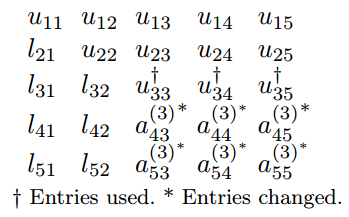
\includegraphics[width=0.49\linewidth]{png/rightlooking.png}
        \hfill
        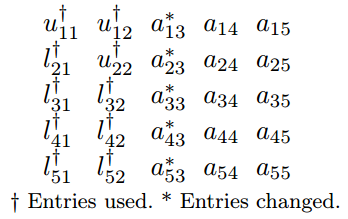
\includegraphics[width=0.49\linewidth]{png/leftlooking.png}
        \caption{Computational sequence for right- and 
        left-looking LU factorization.}
        \label{fig::rightleftlooking}
    \end{figure}

    While the left-looking is more efficient on modern hardware 
    than right-looking, it requires all the columns to the left 
    of the active column to be accessed while it is being 
    updated. Unless the matrix is small, these columns will not 
    fit into the cache, so that access can be slow.
\end{exm}

\subsection{Partial pivoting}
\begin{exm}
    The Gaussian elimination breaks down when $a_{kk}^{(k)}=0$, 
    illustrated by the case
    $$
        \begin{bmatrix}
            0&1\\2&3
        \end{bmatrix}
        \begin{bmatrix}
            x_1\\x_2
        \end{bmatrix}=
        \begin{bmatrix}
            4\\5
        \end{bmatrix}.
    $$ 
    Exchanging the first and second rows completely avoids 
    this difficulty. So at the $k$-th step of Gaussian 
    elimination where $a_{kk}^{(k)}=0$, we have to exchange 
    row $k$ with row $i$ satisfied $i>k$ and $a_{ik}^{(k)}
    \neq 0$. The only way this can break down is if 
    $$
        a_{kk}^{(k)}=a_{k+1,k}^{(k)}=\ldots=a_{nk}^{(k)}=0.
    $$ 
    In this case, $\mA$ is singular and the corresponding 
    equation does not have a unique solution.
\end{exm}

\begin{exm}
    \label{exm::instable}
    Assuming we are solving
    $$
        \begin{bmatrix}
            0.001&2.42\\1.00&1.58
        \end{bmatrix}
        \begin{bmatrix}
            x_1\\x_2
        \end{bmatrix}=
        \begin{bmatrix}
            5.20\\4.57
        \end{bmatrix}
    $$ 
    using a hypothetical computer with a 3-decimal 
    floating-point representation of the form 
    $\pm d_1.d_2d_3\times 10^i$ where $i$ is an integer, 
    $d_1,d_2,d_3$ are decimal digits and $d_1\neq 0$ unless 
    $d_1=d_2=d_3=0$. The triangular system that results from 
    applying Gaussian elimination is
    $$
        \begin{bmatrix}
            0.001&2.42\\0&-2420
        \end{bmatrix}
        \begin{bmatrix}
            x_1\\x_2
        \end{bmatrix}=
        \begin{bmatrix}
            5.20\\-5200
        \end{bmatrix}.
    $$ 
    The computed solution is 
    $$
        \tilde{\mathbf{x}}=\begin{bmatrix}
            \tilde{x}_1\\\tilde{x}_2
        \end{bmatrix}=
        \begin{bmatrix}
            0.00\\2.15
        \end{bmatrix},
    $$
    while the exact solution is
    $$
        \mathbf{x}=\begin{bmatrix}
            x_1\\x_2
        \end{bmatrix}\approx
        \begin{bmatrix}
            1.18\\2.15
        \end{bmatrix}.
    $$
    The error is not small compared with the exact solution.

    However, when we exchange the first and the second row, the 
    factorization will be
    $$
        \begin{bmatrix}
            1.00&1.58\\0.001&2.42
        \end{bmatrix}=
        \begin{bmatrix}
            1\\0.001&1
        \end{bmatrix}
        \begin{bmatrix}
            1.00&1.58\\&2.42
        \end{bmatrix},
    $$ 
    and the computed solution is 
    $$
    \tilde{\mathbf{x}}=\begin{bmatrix}
        \tilde{x}_1\\\tilde{x}_2
    \end{bmatrix}\approx
    \begin{bmatrix}
        1.17\\2.15
    \end{bmatrix},
    $$ 
    which is almost correct.
\end{exm}

\begin{defn}[Partial pivoting]
    One reason why we might get growth that destroys smaller 
    values in the course of the computation comes from having a 
    very large multiplier. A solution to this is to require 
    that the inequality $|l_{ij}|\leq 1$ should hold for the 
    coefficients of the matrix $\mL$. This can be achieved by 
    scanning the $k$-th column below the main diagonal to 
    determine its entry of largest magnitude, the row 
    containing this entry is exchanged with the $k$-th row, 
    therefore $|a_{kk}^{(k)}|\geq |a_{ik}^{(k)}|,\,i>k$ now.
    This strategy is called \textit{partial pivoting}.
\end{defn}

\begin{defn}[Full pivoting]
    At each step in Gaussian elimination, we can choose the 
    pivot to be the largest entry in the remaining submatrix 
    rather than only in the $k$-th row. 
    That is, row and column interchanges are performed at 
    each step to ensure that $|a_{kk}^{(k)}|\geq |a_{ij}^{(k)}|,
    \,i\geq k,j\geq k$ all hold. This strategy is called 
    \textit{full} or \textit{complete pivoting}.
\end{defn}

\begin{thm}
    \label{thm::fullpivot}
    By Gaussian elimination with full pivoting, any nonsingular 
    $\mathbb{R}^{n\times n}$ matrix can be factorized as 
    $\mP\mA\mQ=\mL\mU$, where $\mP$ and $\mQ$ are permutation 
    matrices, $\mL$ is unit lower triangular and  $\mU$ is 
    upper triangular.
\end{thm}
\begin{proof}
    Define elementary permutation matrix $\mI_{pq}$ as the 
    matrix obtained from $\mI$ by exchanging the $p$-th and 
    $q$-th columns (rows). $\mI_{pq}\mA$ exchanges the $p$-th 
    and $q$-th rows of $\mA$ and $\mA\mI_{pq}$ exchanges the 
    $p$-th and $q$-th columns of $\mA$.

    At each step of the full pivoting Gaussian elimination, the 
    row interchange and column interchange can be represented 
    as $\mP_k=\mI_{kp}$ and $\mQ_k=\mI_{kq}$, where $(p,q)$ is 
    the position of the largest entry. So the Gaussian 
    elimination can be represented by
    $$
        \mL_{n-1}\mP_{n-1}\ldots\mL_1\mP_1\mA\mQ_1\ldots\mQ_{n-1}=\mU.
    $$ 
    Define $\mQ=\mQ_1\ldots\mQ_{n-1},\,\mP=\mP_{n-1}\ldots\mP_1,\,
    \mL=\mP(\mL_{n-1}\mP_{n-1}\ldots\mL_1\mP_1)^{-1}$, then we have
    $$
        \mP\mA\mQ=\mL\mU.
    $$ 

    It is obvious that $\mP$ and $\mQ$ are permutation 
    matrices and $\mU$ is upper triangular, so we only need to 
    show $\mL$ is unit lower triangular. Actually $\mL=\mP_{n-1}
    \ldots\mP_2\mL_1^{-1}\mP_2\mL_2^{-1}\ldots\mP_{n-1}\mL_{n-1}^{-1}
    $ because $\mP_k\mP_k=I$. Define
    $$
        \mL^{(1)}=\mL_1^{-1},\,\mL^{(k)}=\mP_k\mL^{(k-1)}\mP_k
        \mL_k^{-1},\,k=2,\ldots,n-1,
    $$  
    then $\mL=\mL^{(n-1)}$. We can verify
    \begin{equation}
        \label{eq::fullpivL}
        \mL^{(k)}=
        \begin{bmatrix}
            \mL_{11}^{(k)}&0\\
            \mL_{21}^{(k)}&\mI_{n-1}
        \end{bmatrix},\,k=1,\ldots,n-1
    \end{equation}
    by induction, where $\mL_{11}^{(k)}$ is a unit lower 
    triangular matrix with entries norm no greater than $1$, 
    $\mL_{21}^{(k)}$ is a $\mathbb{R}^{(n-k)\times k}$ matrix 
    with entries norm no greater than $1$, $\mI_{n-1}$ is the 
    unitary matrix of order $(n-k)$.

    The induction base clearly holds for $k=1$ because of the 
    definition of $\mL^{(1)}=\mL_1^{-1}$. Now suppose that 
    \eqref{eq::fullpivL} holds for $k-1$. Then
    $$
        \mL^{(k)}=\mP_k\mL^{(k-1)}\mP_k\mL_k^{-1}=
        \begin{bmatrix}
            \mL_{11}^{(k-1)}&0\\
            \tilde{\mL}_{21}^{(k-1)}&\tilde{\mL}_k^{-1}
        \end{bmatrix},
    $$ 
    where $\tilde{\mL}_{21}^{(k-1)}$ is obtained from 
    $\mL_{21}^{(k-1)}$ by exchanging its first and $(p-k+1)$-th 
    rows, and
    $$
        \tilde{\mL}_k^{-1}=
        \begin{bmatrix}
            1\\
            l_{k+1,k}&1\\
            l_{k+2,k}&0&1\\
            \vdots&\vdots&\ddots&\ddots\\
            l_{nk}&0&\cdots&0&1
        \end{bmatrix}.
    $$ 
    So \eqref{eq::fullpivL} holds for $k$, which complete the 
    inductive proof.
\end{proof}

\begin{prop}
    Since partial pivoting can be viewed as a special case of 
    full pivoting, any nonsingular $\mathbb{R}^{n\times n}$ 
    matrix can be factorized as $\mP\mA=\mL\mU$, where $\mP$ 
    is a permutation matrix, $\mL$ is unit lower triangular and  $\mU$ is upper triangular.
\end{prop}

\begin{alg}
    By Theorem \ref{thm::fullpivot}, we can still use a single 
    two-dimensional array by writing $\mL$ in the lower 
    triangular part excluding the unit diagonal. The full 
    pivoting Gaussian elimination is then as follows.
    \IncMargin{1em}
    %\LinesNumbered
    \begin{algorithm}[H]
        \caption{Gaussian elimination with full pivoting}
        \SetKwInOut{Precond}{Preconditions}
        \SetKwInOut{Postcond}{Postconditions}

        \KwIn{$\mA\in\mathbb{R}^{n\times n}$}
        \KwOut{$\mathbf{u},\mathbf{v}\in\mathbb{Z}^{n-1}$}
        \Postcond{$\mL$ is stored in the lower triangular part 
        of $\mA$ excluding the unit diagonal, $\mU$ is stored 
        in the upper triangular part of $\mA$, $\mathbf{u}, 
        \mathbf{v}$ record $\mP, \mQ$ seprately}

        \BlankLine
        \For{$k=1,2,\ldots,n-1$}{
            Find $(p,q)$ s.t. $|\mA(p,q)|=\max\{|\mA(i,j)|:
            i=k:n,j=k:n\}$\;
            $\mA(k,1:n)\leftrightarrow \mA(p,1:n)$\;
            $\mA(1:n,k)\leftrightarrow \mA(1:n,q)$\;
            $u(k)=p,\,v(k)=q$\;
            \If{$\mA(k,k)==0$}{
                Full pivoting Gaussian elimination is failed
            }
            $\mA((k+1):n,k)=$ $\mA((k+1):n,k)/\mA(k,k)$\;
            $\mA((k+1):n,(k+1):n)=\mA((k+1):n,(k+1):n)-$ 
            $\mA((k+1):n,k)\mA(k,(k+1):n)$\;
        }
    \end{algorithm}
    \DecMargin{1em}
\end{alg}



\subsection{Block factorization}
\begin{alg}
    \label{exm::blockfactorize}
    In Example \ref{exm::leftlooking}, we show that when the 
    matrix is large, the columns in left-looking method will not 
    fill into the cache, the solution to this problem is to group 
    the updates by blocks. The most useful form is using the 
    left-looking algorithm until a given number $m$ of columns 
    has been factorized, then performing a right-looking block 
    update. If $m$ columns fit into cache, we can factorize the 
    first $m$ columns with one data movement.

    Let us partiation the matrix as
    $$
        \mA=
        \begin{bmatrix}
            \mA_{11}&\mA_{12}\\\mA_{21}&\mA_{22}
        \end{bmatrix},
    $$ 
    where $\mA_{11}$ is of order $m\times m$. Once the 
    processing of the first $m$ columns is complete, we will 
    have the factorization
    $$
        \begin{bmatrix}
            \mA_{11}\\\mA_{21}
        \end{bmatrix}=
        \begin{bmatrix}
            \mL_{11}\\\mL_{21}&\mI
        \end{bmatrix}
        \begin{bmatrix}
            \mU_{11}\\0
        \end{bmatrix}.
    $$ 
    If we had updated the remaining columns, the factorization 
    would have been
    $$
        \begin{bmatrix}
            \mA_{11}&\mA_{12}\\\mA_{21}&\mA_{22}
        \end{bmatrix}=
        \begin{bmatrix}
            \mL_{11}\\\mL_{21}&\mI
        \end{bmatrix}
        \begin{bmatrix}
            \mU_{11}&\mU_{12}\\&\ddot{\mA}_{22}
        \end{bmatrix}.
    $$ 
    By equating corresponding blocks we find the relations
    $$
        \mL_{11}\mU_{12}=\mA_{12},\,\ddot{\mA}_{22}=\mA_{22}-\mL_{21}\mU_{12},
    $$
    $\ddot{\mA}_{22}$ is known as the \textit{Schur complement} 
    of $\mA_{11}$. 

    The columns of $\mU_{12}$ may be found by forward 
    substitution through $\mL_{11}$. The remaining for the 
    given matrix are exactly those that would be made for 
    factorizing the matrix $\ddot{\mA}_{22}$, this can be done 
    by the same strategy.
\end{alg}

\begin{exm}[Implicit block factorization]
    In normal block factorization in Example 
    \ref{exm::blockfactorize}, we calculate 
    \begin{align*}
        &\mA_{11}=\mL_{11}\mU_{11},\\
        &\mL_{11}\mU_{12}=\mA_{12},\\
        &\mL_{21}\mU_{11}=\mA_{21},\\
        &\ddot{\mA}_{22}=\mA_{22}-\mL_{21}\mU_{12}=\mL_{22}
        \mU_{22}.
    \end{align*}
    An interesting variation, known as \textit{implicit block 
    facotrization}, results if the factorization $\mA_{11}=
    \mL_{11}\mU_{11}$ and $\ddot{\mA}_{22}=\mL_{22}\mU_{22}$ 
    are stored, but $\mU_{12}$ is not. When $\mU_{12}$ is 
    needed as a multiplier, $\mL_{11}^{-1}\mA_{12}$ is used 
    instead. This has little merit in the dense case, but in 
    the sparse case it is extremely like that $\mU_{12}$ has 
    many more entries than $\mA_{12}$ so less storage will be 
    needed and sometimes less computation also.
\end{exm}


  
\section{Numerical consideration}
\begin{defn}
    \label{defn::stabledefn}
    To study the effect of arithmetic errors on the solution 
    of sets of questions, we mainly need to answer two 
    questions:
    \begin{enumerate}[(i)]
        \item Is the computed solution $\tilde{\mx}$ the exact 
        solution of a `nearby' problem?
        \item If small changes are made to the given problem, 
        are changes in the exact solution also small?
    \end{enumerate}
    A positive answer to the first question means the error in 
    the computed solution is no greater than what would result 
    from making small pertubations to the original problem and 
    then solving the pertubed problem exactly. In this case, we 
    say that the algorithm is \textit{stable}.

    If the answer to the second question is positive, we say 
    that the problem is \textit{well-conditioned}. Conversly, 
    when small changes in the data produce large changes in the 
    solution, we say the problem is \textit{ill-conditioned}. 
    This is a property of the problem and has nothing to do 
    with the method used to solve it.
\end{defn}

\begin{defn}
    Define the \textit{factorization-error matrix}
    $$
        \mathbf{H}=\tilde{\mL}\tilde{\mU}-\mA,
    $$ 
    where $\tilde{\mL}\tilde{\mU}$ is the numerical 
    factorization of $\mA$.
\end{defn}

\subsection{Controlling algorithm stability through pivoting}
\begin{exm}
    \label{exm::unstable}
    In Example \ref{exm::instable}, we have showed that 
    using Gaussian elimination without pivoting to solve
    $$
        \begin{bmatrix}
            0.001&2.42\\1.00&1.58
        \end{bmatrix}
        \begin{bmatrix}
            x_1\\x_2
        \end{bmatrix}=
        \begin{bmatrix}
            5.20\\4.57
        \end{bmatrix}
    $$ 
    with our hypothetical 3-digit computer cause large error 
    in the solution. Furthermore, the factorization-error 
    matrix
    $$
        \mathbf{H}=
        \begin{bmatrix}
            0.0&0.0\\0.0&-1.58
        \end{bmatrix}
    $$ 
    is not small relative to $\mA$. The residual is
    $$
        \mathbf{r}=\mathbf{b}-\mA\tilde{\mx}=
        \begin{bmatrix}
            -0.003\\1.173
        \end{bmatrix},
    $$ 
    whose norm is not small compared with $\|\mathbf{b}\|$. So 
    we conclude that our algorithm is unstable.

    Note that the damage that lead to the inaccurate 
    factorization is that it treats $1.58$ as zero, the reason 
    that it do so was the large growth in size that take place 
    in forming $a_{22}^{(2)}$ from $a_{22}$.  
\end{exm}

\begin{thm}
    \textit{Backward error analysis} shows that Gaussian 
    elimination is stable provided the growth in Example 
    \ref{exm::unstable} does not take place, actually we 
    have the inequality
    $$
        |h_{ij}|\leq 5.01\epsilon_u n\max_k|a_{ij}^{(k)}|,
    $$ 
    where $\epsilon_u$ is the unit roundoff ($\epsilon_u=0.005$ 
    in our hypothetical 3-digit computer) and $n$ is the 
    dimenson of the matrix. However, it is not practical to 
    control the sizes of all the coefficients $a_{ij}^{(k)}$, 
    we usually weaken the inequality to the bound
    \begin{equation}
        \label{eq::H-bound}
        |h_{ij}|\leq5.01\epsilon_u n\rho,
    \end{equation}
    where
    $$
        \rho=\max_{i,j,k}|a_{ij}^{(k)}|.
    $$ 
\end{thm}
\begin{proof}
    See \cite{Reid1971} combined with our wider bound on 
    rounding error.
\end{proof}

\begin{exm}[Partial pivoting]
    In practice, Gaussian elimination with partial pivoting is 
    considered to be a stable algorithm. This is based on 
    experience rather than rigorous analysis, since the best 
    a priori bound that can be given for a dense matrix is
    $$
        \rho\leq 2^{n-1}\max_{i,j}|a_{ij}|.
    $$ 
    This bound is easy to establish, but generally very 
    pessimistic, particularly in the case where $n$ is very 
    large.
\end{exm}

\begin{exm}[Threshold pivoting]
    While we want to control the size of the multiplier, we 
    may find asking $|a_{kk}^{(k)}|\geq |a_{ik}^{(k)}|,\,i>k$ 
    overly restrictive when other factors need to be taken into 
    account, for example, sparsity or moving data in and out of 
    cache. The compromise strategy is \textit{threshold 
    pivoting} which requires the inequality
    $$
        |a_{kk}^{(k)}|\geq u|a_{ik}^{(k)}|,\,i>k,
    $$ 
    where $u$, the \textit{threshold parameter}, is a value in 
    the range $0<u\leq 1$. Partial pivoting can be regarded as 
    a special threshold pivoting with $u=1$. The growth bound 
    of threshold pivoting is
    $$
        \rho\leq(1+u^{-1})^{n-1}\max_{i,j}|a_{i,j}|.
    $$ 
\end{exm}

\begin{exm}[Rook pivoting]
    Partial pivoting or threshold pivoting only limit the size 
    of the multiplier, however, a small multiplier can produce 
    a relatively large addition to an entry in the lower 
    submatrix if an entry in the row is much larger than the 
    pivot. \textit{Rook pivoting} find the new pivot satisfied
    $$
        |a_{kk}^{(k)}|\geq\max\{|a_{ik}^{(k)}|,|a_{ki}^{(k)}|\},
        \,i>k.
    $$ 
    This limit the size both of the multiplier and the entry in 
    the row. \cite{Foster1997} has shown that, for rook 
    pivoting, the growth is bounded by
    $$
        \rho\leq 1.5n^{3/4\log(n)}\max_{i,j}|a_{i,j}|.
    $$ 
\end{exm}

\begin{exm}[Full pivoting]
    For full pivoting, \cite{Wilkinson1961} has obtained that 
    \begin{align*}
        \rho&\leq f(n)\max_{i,j}|a_{ij}|\\
        &=\sqrt{n(2^13^{1/2}\ldots n^{1/(n-1)})}\max_{i,j}|a_{ij}|.
    \end{align*}
    Note that $f(n)$ is much more smaller than $2^{n-1}$ for 
    large $n$.
\end{exm}

\begin{exm}[SPD case]
    When matrix $\mA$ is SPD, things will be different. 
    \cite{Wilkinson1961} has shown that using Gaussian 
    elimination without pivoting causes no growth i.e.
    $$
        \rho=\max_{i,j,k}|a_{ij}^{(k)}|\leq\max_{i,j}|a_{ij}|.
    $$ 
    So we do not need to consider pivoting when factorize a 
    SPD matrix.
\end{exm}

\begin{exm}[Diagonally dominant case]
    When $\mA$ is diagonally dominant, we can show that
    $$
        \rho=\max_{i,j,k}|a_{i,j}^{(k)}|\leq 
        2\max_{i,j}|a_{i,j}|.
    $$ 
    (Hint: show that $\mA^{(2)}$ is still diagonally dominant 
    and $\sum_{j=2}^n|a_{ij}^{(2)}|\leq\sum_{j=1}^n|a_{ij}|$.)
\end{exm}

\subsection{Monitoring the stability}
\begin{defn}
    Since it is easy to compute $\mathbf{r}=\mathbf{b}-\mA\mx$, 
    and in practice this measure for the stability of the 
    solution is usually employed. We mainly compare 
    $\|\mathbf{r}\|$ with $\|\mathbf{b}\|$ or $\|\mA\|
    \|\tilde{\mx}\|$ to monitor the stability.

    If $\|\mathbf{r}\|$ is small compared with $\|\mathbf{b}\|$, 
    then we have solved a nearby problem since $\mA\tilde{\mx}=
    \mathbf{b}-\mathbf{r}$. By the first question in Definition 
    \ref{defn::stabledefn}, our method is stable.

    If $\|\mathbf{r}\|$ is small compared with $\|\mA\|
    \|\tilde{\mx}\|$, then $\tilde{\mx}$ is the exact solution 
    of the equation $(\mA+\mathbf{H})\tilde{\mx}=\mathbf{b}$ 
    where $\|\mathbf{H}\|$ is small compared with $\|\mA\|$. 
    By the first question in Definition \ref{defn::stabledefn}, 
    our method is stable.

    Thus, if $\|\mathbf{r}\|$ is small compared with 
    $\|\mathbf{b}\|$, $\|\mA\tilde{\mx}\|$, or $\|\mA\|
    \|\tilde{\mx}\|$, we have done a good job in solving the 
    equation.
\end{defn}

\subsection{Ill-conditioning}
\begin{exm}
    Suppose the matrix $\mA$ is ill-conditioned, for example, 
    there are two vector $\mathbf{v}$ and $\mathbf{w}$ 
    satisfied
    $$
        \|\mathbf{v}\|=\|\mathbf{w}\|,\,\|\mA\mathbf{v}\|
        \gg \|\mA\mathbf{w}\|.
    $$ 
    $\mathbf{v}$ is the solution of $\mA\mx=\mathbf{b}$, where 
    $\mathbf{b}=\mA\mathbf{v}$. Now we change $\mathbf{b}$ by 
    the vector $\mA\mathbf{w}$ which is relatively small but 
    the corresponding solution changes a lot. 

    Clearly, the amount of ill-conditioning is dependent on 
    $\|\mA\mathbf{v}\|/\|\mA\mathbf{w}\|$, this ratio can be 
    written in the form
    $$
        \frac{\|\mA\mathbf{v}\|}{\|\mA\mathbf{w}\|}=
        \frac{\|\mA\mathbf{v}\|}{\|\mA\mathbf{w}\|}
        \frac{\|\mathbf{w}\|}{\|\mathbf{v}\|}=
        \frac{\|\mA\mathbf{v}\|}{\|\mathbf{v}\|}
        \frac{\|\mA^{-1}\mathbf{y}\|}{\|\mathbf{y}\|},
    $$ 
    where $\mathbf{y}=\mA\mathbf{w}$. The right hand side has 
    an upper bound $\|\mA\|\|\mA^{-1}\|$.
\end{exm}

\begin{defn}[Condition number]
    The quantity
    $$
        \kappa(\mA)=\|\mA\|\|\mA^{-1}\|
    $$ 
    is known as the \textit{condition number} of $\mA$.
\end{defn}

\begin{thm}
    For the general problem $\mA\mx=\mathbf{b}$, we consider 
    its backward error. Assume $\mathbf{b}$ is perturbed by 
    $\mathbf{\delta b}$ and the corresponding pertubation of 
    $\mx$ is $\mathbf{\delta x}$ so that equation
    $$
        \mA(\mx+\mathbf{\delta x})=\mathbf{b}+\mathbf{\delta b}
    $$ 
    holds. Then the relative error can be controlled by
    $$
        \frac{\|\mathbf{\delta x}\|}{\|\mx\|}\leq \kappa(\mA)
        \frac{\|\mathbf{\delta b}\|}{\|\mathbf{b}\|}.
    $$ 
\end{thm}

\begin{thm}
    Now we consider the backward error for the matrix term. 
    Let the perturbed equation be
    $$
        (\mA+\mathbf{\delta A})(\mx+\mathbf{\delta x})=
        \mathbf{b}.
    $$ 
    Then the relative error can be controlled by
    $$
        \frac{\|\mathbf{\delta x}\|}{\|\mx+\mathbf{\delta x}\|}
        \leq \kappa(\mA)\frac{\|\mathbf{\delta A}\|}{\|\mA\|}.
    $$ 
\end{thm}

\begin{thm}
    When we consider the perturbation of $\mA$ and $\mathbf{b}$ 
    at the same time, we have the equation
    $$
        (\mA+\mathbf{\delta A})(\mx+\mathbf{\delta x})=
        \mathbf{b}+\mathbf{\delta b}.
    $$ 
    When $\|\mA^{-1}\|\|\mathbf{\delta A}\|<1$, we have
    $$
        \frac{\|\mathbf{\delta x}\|}{\|\mx\|}
        \leq \frac{\kappa(\mA)}{1-\kappa(\mA)
        \frac{\|\mathbf{\delta A}\|}{\|\mA\|}}
        \left[\frac{\|\mathbf{\delta b\|}}{\|\mathbf{b}\|}
        +\frac{\|\mathbf{\delta A}\|}{\|\mA\|}\right].
    $$ 
\end{thm}
\begin{proof}
    \begin{align*}
        &(\mA+\mathbf{\delta A})(\mx+\mathbf{\delta x})=
        \mathbf{b}+\mathbf{\delta b},\\
        \Rightarrow&\mA\mathbf{\delta x}=\mathbf{\delta b}
        -\mathbf{\delta A}\mx-\mathbf{\delta A}
        \mathbf{\delta x},\\
        \Rightarrow&\|\mathbf{\delta x}\|\leq\|\mA^{-1}\|
        (\|\mathbf{\delta b}\|+\|\mathbf{\delta A}\|\|\mx\|
        +\|\mathbf{\delta A}\|\|\mathbf{\delta x}\|),\\
        \Rightarrow&\|\mathbf{\delta x}\|(1-\|\mA^{-1}\|
        \|\mathbf{\delta A}\|)\\&\leq \|\mA^{-1}\|(\|
        \mathbf{\delta b}\|+\|\mathbf{\delta A}\|\|\mx\|).
    \end{align*}
    Provided the inequality $\|\mA^{-1}\|\|\mathbf{\delta A}\|
    <1$ holds, we deduce the relation
    $$
        \|\mathbf{\delta x}\|\leq\frac{\|\mA^{-1}\|}
        {1-\|\mA^{-1}\|\|\mathbf{\delta A}\|}(\|
        \mathbf{\delta b}\|+\|\mathbf{\delta A}\|\|\mx\|)
    $$ 
    for the absolute error. For the relative error, we divide 
    this by $\|\mx\|$ and use the inequality $\|\mathbf{b}\|
    \leq\|\mA\|\|\mx\|$ to give the inequality
    $$
    \frac{\|\mathbf{\delta x}\|}{\|\mx\|}
    \leq \frac{\kappa(\mA)}{1-\kappa(\mA)
    \frac{\|\mathbf{\delta A}\|}{\|\mA\|}}
    \left[\frac{\|\mathbf{\delta b\|}}{\|\mathbf{b}\|}
    +\frac{\|\mathbf{\delta A}\|}{\|\mA\|}\right].
    $$ 
\end{proof}

\begin{defn}[Scaling]
    \textit{Scaling} is to select two diagonal matrices 
    $\mathbf{D}_1$ and $\mathbf{D}_2$ such that
    $\mathbf{D}_1\mA\mathbf{D}_2$
    has a smaller condition number than $\mA$.
\end{defn}

\begin{exm}
    \label{exm::conditionnum}
    The condition number is very dependent on scaling. Consider 
    the identity matrix with the last diagonal entry replaced 
    by a small number $\delta$, then $\kappa(\mA)$ will be 
    around $1/\delta$. However, if the matrix is scaled to make 
    its last entry $1$, the condition number of the scaled 
    matrix is just $1$.
\end{exm}

\subsection{Strategies to improve the accuracy}
\begin{alg}[Iterative refinement]
    Let $\mx^{(1)}$ be the computed solution to $\mA\mx=
    \mathbf{b}$, let the residual vector be
    $$
        \mathbf{r}^{(1)}=\mathbf{b}-\mA\mx^{(1)}.
    $$ 
    Formally, we observe the relations
    $$
        \mA^{-1}\mathbf{r}^{(1)}=\mA^{-1}\mathbf{b}-\mx^{(1)}
        =\mx-\mx^{(1)}.
    $$ 
    Hence, we may find a correction $\Delta\mx^{(1)}$ to $\mx$ 
    by solving 
    $$
        \mA\Delta\mx^{(1)}=\mathbf{r}^{(1)}.
    $$ 
    In practive, of course, we can not solve this exactly, but 
    we may construct a new approximation solution
    $$
        \mx^{(2)}=\mx^{(1)}+\Delta \mx^{(1)},
    $$ 
    and, in general, define an iteration with steps
    \begin{align*}
        &r^{(k)}=\mathbf{b}-\mA\mx^{(k)},\\
        &\textrm{solve}\quad\mA\Delta \mx^{(k)}=\mathbf{r}^{(k)},\\
        &\mx^{(k+1)}=\mx^{(k)}+\Delta\mx^{(k)},
    \end{align*}
    for $k=1,2,\ldots\,$.
\end{alg}

\begin{alg}[Automatic scaling]
    \label{alg::autoscale1}
    A practical automatic scaling algorithm is to make all 
    entries are close to $1$. Let $\mathbf{D}_1=
    \mathrm{diag}(e^{-\rho_i})$ and $\mathbf{D}_2=\mathrm{diag}
    (e^{-\gamma_j})$, where $\rho_i$ and $\gamma_i,\,i=1,2,\ldots,
    n$ are chosen to  minimize
    \begin{equation}
        \label{eq::scalinglog}
        \sum_{a_{ij}\neq 0}(\log|a_{ij}|-\rho_i-\gamma_j)^2.
    \end{equation}
    Then $\mathbf{D}_1\mA\mathbf{D}_2$ has the logarithms of 
    its nonzeros as small as possible in the least-squares 
    sense. The minimization of \eqref{eq::scalinglog} is a 
    linear least-squares problem, which can be solved 
    effectively by CG.
\end{alg}

\begin{alg}[Automatic scaling]
    \label{alg::autoscale2}
    Another approach to scaling is to use an iterative 
    technique to make the infinity norms of all the rows and 
    columns close to one. \cite{Ruiz2014} acheive this by 
    repeatedly scaling the rows and columns by the square roots 
    of their norms. Starting with $\mA^{\{0\}}=\mA$ and 
    $$
        a_{ij}^{\{k+1\}}=\|a_{i:}^{\{k\}}\|_\infty^{-1/2}
        a_{ij}^{\{k\}}\|a_{:j}^{\{k\}}\|_\infty^{-1/2}.
    $$ 
    Since any element of $\mA^{\{k\}}$ is less than the norm of 
    its row or column, all entries of $\mA^{\{k\}},\,k\geq 1$ 
    are less than $1$ in absolute value. If $a_{il}^{\{k\}}$ is 
    the largest entry in row $i$, then
    $$
        |a_{il}^{\{k+1\}}|=\|a_{i:}^{\{k\}}\|_\infty^{1/2}
        \|a_{:l}^{\{k\}}\|_\infty^{-1/2}\geq
        \|a_{i:}^{\{k\}}\|_\infty^{1/2}.
    $$ 
    It follows that the norm of row $i$ converge to $1$ because
    $$
        \|a_{i:}^{\{k+1\}}\|_\infty\geq
        \|a_{i:}^{\{k\}}\|_\infty^{1/2}\geq
        \|a_{i:}^{\{k\}}\|_\infty.
    $$ 
    A similar results applies for the columns. Ruiz stops the 
    iteration when
    \begin{align*}
        &\max_{1\leq i\leq n}\left|1-\|a_{i:}^{\{k\}}\|_\infty
        \right|\leq\epsilon \,\mathrm{and} \\
        &\max_{1\leq j\leq n}\left|1-\|a_{:j}^{\{k\}}\|_\infty
        \right|\leq\epsilon.
    \end{align*}
\end{alg}

\begin{exm}
    For the matrix
    $$
        \mA=
        \begin{bmatrix}
            1.00&2420\\1.00&1.58
        \end{bmatrix},
    $$ 
    the algorithm \ref{alg::autoscale1} yields the scaled matrix
    $$
        \mathbf{D}_1\mA\mathbf{D}_2=
        \begin{bmatrix}
            0.1598&6.2559\\6.2559&0.1598
        \end{bmatrix}.
    $$ 
    The algorithm \ref{alg::autoscale2} yields the scaled matrix
    $$
    \mathbf{D}_1\mA\mathbf{D}_2=
    \begin{bmatrix}
        0.0228&1\\1&0.0286
    \end{bmatrix}.
    $$ 
\end{exm}
%%% Local Variables:
%%% mode: latex
%%% TeX-master: "LU_MathDocument"
%%% End:



\section{Orderings in sparse Gaussian elimination}
\label{sec:OrderingInSparse}

\subsection{Orderings}
\label{sec:orderings}

\begin{exm}
  \label{exm:reordering}
  Consider the matrix that has the pattern illustrated on the right of
  Figure \ref{fig:ReorderingSparse} with diagonal entries $1.0$ and
  off-diagonal entries $1.1$. The partial pivoting strategy would
  destroy all sparsity because none of the diagonal entries would be
  available as a pivot. However, if we adapt the threshold pivoting
  strategy with $u=0.1$ to the sparse case,  all the
  diagonal entries except the last are available as pivots and the
  sparsity is well preserved.

  \begin{figure}[H]
    \centering
    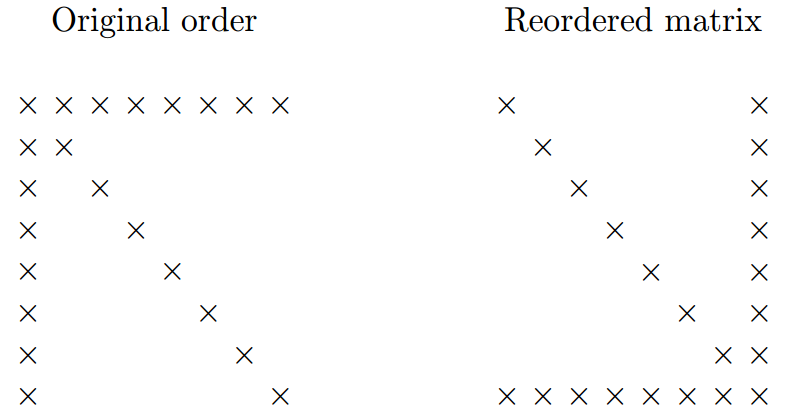
\includegraphics[width=7cm]{png/ReorderingSparse.png}
    \caption{Reordering can preserve sparsity in factorization.}
    \label{fig:ReorderingSparse}
  \end{figure}
\end{exm}

\begin{rmk}
  Ordering the rows and columns to preserve sparsity in Gaussian
  elimination was demonstrated to be effective in the Example
  \ref{exm:reordering}.
  There are four quite different strategies for ordering a sparse
  matrix which are introduced in the following section:
  \begin{enumerate}
  \item We may be able to reorder the matrix to block
    triangular form. We discuss this in Section \ref{sec:GEforSM}. If
    such an ordering exists, we can confine the factorization steps to
    smaller blocks on the diagonal, rather than to the whole matrix.
  \item We consider local strategies where, at each stage of
    the factorization, we choose as pivot the entry that preserves
    sparsity "as well as possible" according to some criteria, which
    will be introduced in Section \ref{sec:LocalPivotal}.
  \item There are methods of preserving sparsity by confining
    fill-ins to particular areas of the matirx, which will be
    developed in Section \ref{sec:BandSolution}.
  \item A strategy under the heading of dissection methods
    looks at the matrix in its entirety, seeking to split the overall
    problem into independent subproblems, which is particularly
    applicable for parallel computing environments. We will discuss in
    Section \ref{sec:Dissection}.
  \end{enumerate}

  There is no single "best" method for preserving sparsity. The
  criteria for what is best is more difficult than it might seem at
  first. For example, the criterion of "least fill-in" might seem to
  be best, but may require a great deal more data structure
  manipulation. 
\end{rmk}
\subsection{Reduction to block triangular form}
\label{sec:GEforSM}
 
\begin{defn}
  \label{defn:BLTF}
  A pattern is worthwhile to seek is the \emph{block lower triangular form}
  \begin{equation}
    \label{eq:BLTF}
    \mathbf{PAQ}=\left[
    \begin{array}{ccccc}
      \mathbf{B}_{11}& & & & \\
     \mathbf{ B}_{21} & \mathbf{B}_{22} & & & \\
      \mathbf{B}_{31} & \mathbf{B}_{32} &\mathbf{B}_{33} & & \\
      \vdots&\vdots&\vdots&\ddots& \\
      \mathbf{B}_{N1}& \mathbf{B}_{N2}& \mathbf{B}_{N3} & \cdots& \mathbf{B}_{NN}\\
    \end{array}
  \right]
  \end{equation}
\end{defn}

\begin{defn}
  A matrix that can be permuted to the form \eqref{eq:BLTF}, with
  $N>1$, is said to be \emph{reducible}. If no block triangular form
  other than the trivial one can be found, the matrix is called
  \emph{irreducible}. We expect each $\mathbf{B}_{ii}$ to be irreducible, for
  otherwise a finer decomposition is possible.
\end{defn}

\begin{alg}
  If we partition $\mathbf{x}$ and $\mathbf{b}$ similarly, we may solve the equation
  $\mathbf{Ax=b}$ by solving the simple forward substitution.
  \begin{equation}
    \label{eq:BLTFSolving}
    \mathbf{B}_{ii}\mathbf{y}_i=(\mathbf{Pb})_i-\sum\limits_{j=1}^{i-1}\mathbf{B}_{ij}\mathbf{y}_j,\
    i=1,2,\ldots,N 
  \end{equation}
  and the permutation
  \begin{equation}
    \label{eq:PermutationYtoX}
    \mathbf{x=Qy}.
  \end{equation}
\end{alg}

\begin{rmk}
  We have to factorize only the
  diagonal blocks $\mathbf{B}_{ii}$. The off-diagonal blocks $\mathbf{B}_{ij},\ i>j$,
  are used only in the multiplications $\mathbf{B}_{ij}\mathbf{y}_j$. In particular, all
  fill-in is confined to the blocks on the diagonal. Any row and
  column interchanges needed for the sake of stability and sparsity
  may be performed within the blocks on the diagonal and do not affect
  the block triangular structure.
\end{rmk}

\begin{alg}
  We may find the block triangular form in three stages:
  \begin{enumerate}[(i)]
  \item Look for row and column singletons.
  \item Permute entries onto the diagonal (usually called finding a
    \emph{transversal}).
  \item Use symmetric permutations to find the block form itself.
  \end{enumerate}
  In this section, we discuss the three stages separately.
\end{alg}

\begin{alg}
  When we look for row and column singletons,
  \begin{enumerate}[(i)]
  \item If the matrix has a row singleton and we permute it to the
    position $(1,1)$, the matrix has the form
    $$\mathbf{PAQ}=\left[
      \begin{array}{cc}
        \mathbf{B}_{11}& \\ \mathbf{B}_{21} & \mathbf{B}_{22}
      \end{array}
    \right]$$ where $\mathbf{B}_{11}$ has order $1$. If the matrix $\mathbf{B}_{22}$has
    a row singleton, we may permute it to the position
    $(2,2)$. Continuing in this way until no row singletons are
    available, we find the permuted form with $\mathbf{B}_{11}$ a lower
    triangular matrix.
  \item Similarly, we may look for column singletons successively and
    permute each in turn to the end of the matrix. Following this we
    have the form
     $$\mathbf{PAQ}=\left[
      \begin{array}{ccc}
        \mathbf{B}_{11}& & \\ \mathbf{B}_{21} & \mathbf{B}_{22} & \\
        \mathbf{B}_{31} & \mathbf{B}_{32} & \mathbf{B}_{33}
      \end{array}\right]
      $$ where $\mathbf{B}_{11}$ and $\mathbf{B}_{33}$ are lower triangular matices.
    \end{enumerate}
  \end{alg}

  \begin{exm}
    We show an example in Figure \ref{fig:Singletons}. There is one
    row singleton and choosing it creates another. There are two
    column singletons and choosing them creates another. We are left
    with a middle block of size $2$.
    
    \begin{figure}[H]
    \centering
    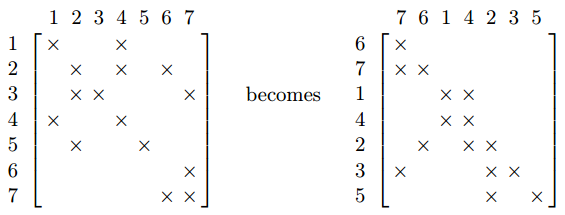
\includegraphics[height=3cm]{png/Singletons.png}
    \caption{Permuting row and column singletons.}
      \label{fig:Singletons}
  \end{figure}
\end{exm}

\begin{rmk}
  In the rest of the section, we consider how $\mathbf{B}_{22}$ can be permuted
  to block triangular form.
\end{rmk}


\begin{defn}
  The algorithm of finding a transversal can be described in either a
  row or a column orientation. We follow the variant that looks at the
  columns one by one and permutes the rows.
  After permutations have been found that place entries in the first
  $k-1$ diagonal positions, we examine column $k$ and seek a row
  permutation that will:
  \begin{enumerate}[(i)]
  \item Preserve the presence of entries in the first $k-1$ diagonal
    positions,
  \item result in column $k$ having an entry in row $k$.
  \end{enumerate}
  The algorithm continues in this fashion extending the transversal by one at
  each stage. Success in this extension is called an
  \emph{assignment}. Sometimes this transversal extension step is
  trivial, which is called a \emph{cheap assignment}.
\end{defn}

\begin{exm}
  In Figure \ref{fig:CheapA}, the assignment in column six is made by
  the interchange of rows six and seven. Figure \ref{fig:NotCheapA}
  shows a simple case where a cheap assignment is not available, but
  the interchange of rows one and seven is adequate the $(1,1)$ entry
  and make a cheap assignment possible in column six.
  \begin{figure}[H]
  \centering
  \subfigure[A cheap assignment for column 6]{
    \label{fig:CheapA}
    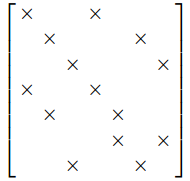
\includegraphics[width=3cm]{png/CheapAssignment.png}
  }
  \hspace{1cm}
  \subfigure[A single preliminary row interchange is needed]{
    \label{fig:NotCheapA}
    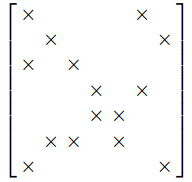
\includegraphics[width=3cm]{png/NotCheapAssignment.png}}
  \caption{Two examples of assignment.}
  \label{fig:Assignment}
\end{figure}
\end{exm}

\begin{defn}
  Sometimes the transversal cannot be extended because the matrix is
  singular for all numerical values of the entries. Such a matrix is
  called \emph{symbolically singular} or \emph{structurally singular}.
\end{defn}

\begin{exm}
  A symbolically singular case is
  $$\left[
    \begin{array}{ccccc}
      \times & \times & & \times & \\
             & & \times & & \times\\
      & & \times & & \times\\
      \times & \times & & \times & \\
      & & \times & & \times\\
    \end{array}
  \right].$$
\end{exm}

\begin{alg}[Transversal extension by depth-first search]
  \label{algo:DFSforTransversal}
  We seek a sequence of columns $c_1,c_2,\ldots,c_j$ with
  $c_1=k$ having entries in rows $r_1,r_2,\ldots,r_j$, with
  $r_i=c_{i+1},\ i=1,2,\ldots,j-1$ and $r_j\geq k.$ Then the sequence of
  row interchanges $(r_1,r_2),\ldots,(r_{j-1},r_j)$ achieves what we
  need. To find this we start with the first entry in column $k$ we take
  its row number to indicate the next column and continue letting the
  first off-diagonal entry in each column indicate the subsequent
  column. In each column, we look for an entry in row $k$ or
  beyond. This sequence has one of the following possible outcomes:
  \begin{enumerate}[(i)]
  \item We find a column with an entry in row $k$ or beyond.
  \item We reach a row already considered.
  \item We come to a dead end (that is a column with no off-diagonal
    entries or one whose off-diagonal entries have all already been considered).
  \end{enumerate}
  In case (i) we have the sequence of columns that we need. In case
  (ii) we take the next entry in the current column. In case (iii), we
  backtrack to the previous column and start again with the next entry there.
\end{alg}

\begin{exm}
  In figure \ref{fig:NotCheapA}, we seek a sequence of
  columns $6,1,7$ by the above algorithm, so the interchange of rows 1
  and 7 is adequate to preserve the $(1,1)$ entry and make a cheap
  assignment possible in column 6. 
\end{exm}

\begin{rmk}
  Always taking the next column rather than trying other rows in the present
column is the depth-first part. Looking to see if there is an entry in 
row k or  beyond is the look-ahead feature.
\end{rmk}
\begin{thm}
  If the matrix order is $n$ and it has $\tau$ entries, the number of elementary
  operations of algorithm~\ref{algo:DFSforTransversal} is at worst proportional to $n\tau$.
\end{thm}

\begin{rmk}
  We assume that a row permutation $\mathbf{P}_1$ has been computed so that
  $\mathbf{P}_\mathbf{1A}$ has entries on every position on its diagonal, then we wish
  to find a permutation matrix $\mathbf{Q}$ such that $\mathbf{Q}^T(\mathbf{P}_1\mathbf{A})\mathbf{Q}$ has the form
  \begin{equation}
    \mathbf{Q^T}(\mathbf{P}_1\mathbf{A})\mathbf{Q}=\left[
    \begin{array}{ccccc}
      \mathbf{B}_{11}& & & & \\
      \mathbf{B}_{21} & \mathbf{B}_{22} & & & \\
      \mathbf{B}_{31} & \mathbf{B}_{32} & \mathbf{B}_{33} & & \\
      \vdots&\vdots&\vdots&\ddots& \\
      \mathbf{B}_{N1}& \mathbf{B}_{N2}& \mathbf{B}_{N3} & \cdots& \mathbf{B}_{NN}\\
    \end{array}
  \right]
  \end{equation}
\end{rmk}

\begin{rmk}
  It is convenient to describe algorithms for this process with the
  help of the directed graphs associated with the matrices. Applying a
  symmetric permutation to the matrix causes no change in the
  associated directed graph except for the relabelling of its nodes.
\end{rmk}

\begin{thm}
  \label{thm:Divide2Part}
  If we cannot find a closed path, we must be able to divide the
  directed graph into two parts such that there is no path from the
  first part to the second. Renumbering the first group of nodes
  $1,2,\ldots,k$ and the seconde group $k+1,\ldots,n$ will produce a
  corresponding matrix in block lower triangular form.
\end{thm}

\begin{defn}
The same process in theorem \ref{thm:Divide2Part} may be applied to
each resulting block until no fuether subdivision is possible. The
sets of nodes corresponding to the resulting diagonal blocks are
called \emph{strong components}.  
\end{defn}

\begin{exm}
  In Figure \ref{fig:SymPermToBTF}, there is no connection from nodes $(1,2)$ to nodes
  $(3,4,5)$. The corresponding matrix is of block lower triangular
  form.
  \begin{figure}[H]
    \centering
    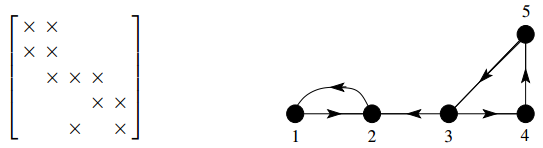
\includegraphics[width=8cm]{png/SymPermToBTF.png}
    \caption{A $5\times 5$ matrix and its digraph(directed graph).}
    \label{fig:SymPermToBTF}
  \end{figure}
\end{exm}

\begin{thm} \label{thm:Sargent}
  If $\mathbf{A}$ is a symmetric permutation of a triangular matrix, there must
  be a node in its digraph from which no path leaves.
\end{thm}

\begin{alg}
  \label{algo:FindingTF}
  The algorithm for finding the triangular form may be built upon the
  theorem \ref{thm:Sargent}:
  \begin{enumerate}
  \item We may start anywhere in the digraph and trace a path until we
    encounter a node from which no paths leave,
  \item number the node at the end of the path first, and remove it
    and all edges pointing to it from the digraph,
  \item continue from the previous node on the path until once again
    we reach a node with no path leaving it.
  \end{enumerate}
\end{alg}

\begin{exm}
  We illustrate the algorithm with the digraph of Figure \ref{fig:DigraphOfSargent}. The
  sequence of paths is illustrated in Figure \ref{fig:AlgorithmOfSargent}.
  \begin{figure}[H]
    \centering
    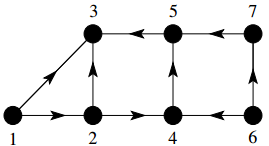
\includegraphics[width=4cm]{png/DigraphToTri.png}
    \caption{A digraph corresponding to a triangular matrix}
    \label{fig:DigraphOfSargent}
  \end{figure}
   \begin{figure}[H]
     \centering
    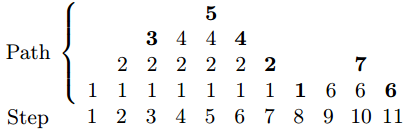
\includegraphics[width=6cm]{png/SequenceOfAlgoSW.png}
    \caption{The sequence of paths used for the Figure
      \ref{fig:DigraphOfSargent} case, where nodes selected for
      ordering are shown in bold.}
     \label{fig:AlgorithmOfSargent}
  \end{figure}
\end{exm}

\begin{defn}
  \emph{A composite node} denotes any group of nodes through which a
  closed path has been found. Edges within a composite node are ignored,
and edges entering or leaving any node of the composite node are regarded as
entering or leaving the composite node. It generalized the idea of
  algorithm~\ref{algo:FindingTF} to the block case.
\end{defn}

\begin{alg}[The algorithm of Sargent and Westerberg]
  
  Starting from any node, a path is followed through the digraph
  until:
  \begin{enumerate}
  \item A closed path is found (identified by encountering the same
    node or composite node tweice), or
  \item a node or composite node is encountered with no edges leaving it.
  \end{enumerate}
  In case (i), all the nodes on the closed path must belong to the same strong
component and the digraph is modified by collapsing all nodes on the closed
path into a single composite node.  The path is now continued from the
composite node.
In case (ii), as for ordinary nodes in the triangular case, the composite node
is numbered next in the relabelling. It and all edges connected to it are removed,
and the path now ends at the previous node or composite node, or starts from
any remaining node if it would otherwise be empty.
\end{alg}

\begin{exm}
   \begin{figure}[H]
    \centering
    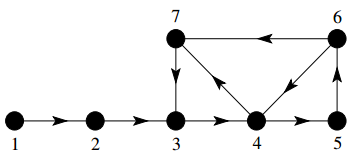
\includegraphics[width=5cm]{png/DigraphToBTri.png}
    \caption{A digraph illustrating the algorithm of Sargent and
      Westerberg.}
    \label{fig:DigraphToBTri}
  \end{figure}
   \begin{figure}[H]
     \centering
    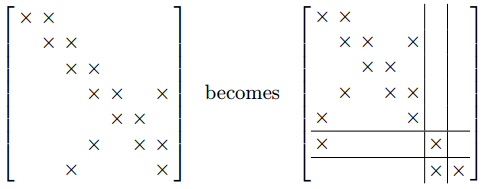
\includegraphics[width=6cm]{png/SequenceOfAlgoSW2.png}
    \caption{The matrices before and after renumbering.}
    \label{fig:MatricesChange}
  \end{figure}
  We illustrate with the example shown in Figure
  \ref{fig:MatricesChange}. Starting the path at node 1, it continues
  $1 \rightarrow 2\rightarrow 3\rightarrow 4\rightarrow 5\rightarrow
  6\rightarrow 4$, then $(4,5,6)$ is recognized as a closed path, and
  nodes 4,5,6 are relabelled as composite node $4'$. The path is
  continued from this composite node to become $1\rightarrow
  2\rightarrow 3\rightarrow 4'\rightarrow 7\rightarrow 3$. Again, a
  closed path has been found and $(3,4',7)$ is labelled as $3'$ and
  the path becomes $1\rightarrow 2\rightarrow 3'.$ Since there are no
  edges leaving $3'$, it is numbered first and removed. The path is
  now $1\rightarrow 2$ and no edges leave node 2, so this is numbered
  second. Finally, node 1 is numbered as the last block. The
  corresponding original and reordered matrices are shown in Figure
  \ref{fig:MatricesChange}.
\end{exm}

\begin{rmk}
  The difficulty with this approach is that there may be large
  overheads associated with the relabelling in the node collapsing
  step. A simple scheme such as labelling each composite node with the
  lowest label of its constituent nodes can result in $\mathcal{O}(n^2)$ relabellings.
\end{rmk}

\begin{exm}
  In Figure successive composite nodes are (4, 5), (3, 4, 5, 6), (2, 3,
  4, 5, 6, 7), (1, 2, 3, 4, 5, 6, 7, 8). In general, such a digraph
  with $n$ nodes will involve $2+4+6+\cdots+n=n^2/4+n/2$ relabellings.
\begin{figure}[H]
  \centering
    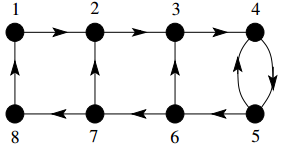
\includegraphics[width=5cm]{png/ManyRelabelling.png}
    \caption{A case causing many relabellings.}
    \label{fig:ManyRelabelling}
  \end{figure}
\end{exm}

\subsection{Local pivotal strategies for sparse matrices}
\label{sec:LocalPivotal}

\begin{defn}
  Suppose Gaussian elimination applied to an $n\times n$ matrix has
  proceeded through the first $k-1$ stages. For each row $i$ in the
  active $(n-k+1)\times(n-k+1)$ submatrix, let $r_i^{(k)}$ denotes the
  number of entries in row $i$. Similarly, let $c_j^{(k)}$ be the
  number of entries in column $j$. Then, the Markowitz criterion is to
  select the entry $a_{ij}^{(k)}$ that minimizes the expression
  \begin{equation}
    \label{eq:MarkowitzCriterion}
    (r_i^{(k)}-1)(c_j^{(k)}-1)
  \end{equation}
  from the entries of the active $(n-k+1)\times(n-k+1)$ submatrix that
  are not too small numerically.
\end{defn}

\begin{rmk}
  An advantage of using \eqref{eq:MarkowitzCriterion} rather than
  $r_i^{(k)}c_j^{(k)}$ is that this forces the algorithm to select a
  row singleton or a column singleton if either is present. Such a
  choice produces no fill-in at all.
\end{rmk}

\begin{thm}
 If $\mathbf{A}$ is symmetric,  the search for the pivot is simplified to
 finding $i$ such that $$r_i^{(k)}=\min\limits_tr_t^{(k)}$$ leading to
 $a_{ii}^{(k)}$ as pivot if $a_{ii}^{(k)}$ is nonzero.
\end{thm}
\begin{rmk}
  It is called the minimum degree algorithm because of its graph
  theoretic interpretation: in the graph assoiated with a symmetric
  sparse matrix, this strategy corresponds to choosing the node for
  the next elimination that has the least edges connected to it.
\end{rmk}

\begin{alg}
  Assoicated with the Markowitz ordering strategy is the need in the
  unsymmetric case to establish a suitable threshold parameter, $u$,
  for numerical stability. In particular, we restrict the Markowitz
  selection to those pivot candidates satisfying the inequality
  \begin{equation}
    \label{eq:MarkowitzThreshold}
    |a_{kk}^{(k)}|\geq u|a_{ik}^{(k)}|,\ i>k,
  \end{equation}
  where $u$ is a preset parameter in the range $0<u\leq 1$.
\end{alg}

\subsection{Ordering sparse mtrices for band solution}
\label{sec:BandSolution}

\begin{rmk}
We consider a different approach to reordering to preserve sparsity,
with algorithms that take a global view of the problem.
\end{rmk}


\begin{defn}
 A sparse matrix in which the nonzero elements are located in a band
 about the main diagonal is called a \emph{band matrix}. If $\mathbf{A}$ is a band matrix, then
 $$a_{ij}=0,\ |i-j|>s \mbox{ for some value } s,$$
 which is illustrated on the left of Figure \ref{fig:bandedMatrix}.
\end{defn}

\begin{defn}
  For a symmetrically structured matirx $\mathbf{A}$ has \emph{bandwidth} $2m+1$ and
  \emph{semibandwidth} $m$ if $m$ is the smallest integer such that
  $a_{ij}=0$ whenever $|i-j|>m.$ For unsymmetric case, we define the
  lower (upper) semibandwidth as the smallest integer $m_l (m_u)$ such
  that if $a_{ij}$ is an entry, $i-j\leq m_l$ ($j-i\leq m_u$). The
  bandwidth is $m_l+m_u+1.$
\end{defn}

\begin{defn}
  $\mathbf{A}$ is of the \emph{variable-band} form (also called skyline form) if
  $$a_{ij}=0,\ j-i>s_i \mbox{ or } a_{ji}=0,\ j-i>t_i$$
  for some values $s_i$ and $t_i,\ i=1,2,\ldots,n$, which is shown on
  the right of Figure \ref{fig:bandedMatrix}.
\end{defn}

\begin{defn}
  When using the variable-band form for a symmetric matrix, we store
  for each row every coefficient between the first entry in the row
  and the diagonal. In the unsymmetric case, we also store for each
  column every coefficient between the first entry in the column and
  the diagonal. The total number of coefficients stored is called the \emph{profile}.
\end{defn}

\begin{figure}[H]
  \centering
    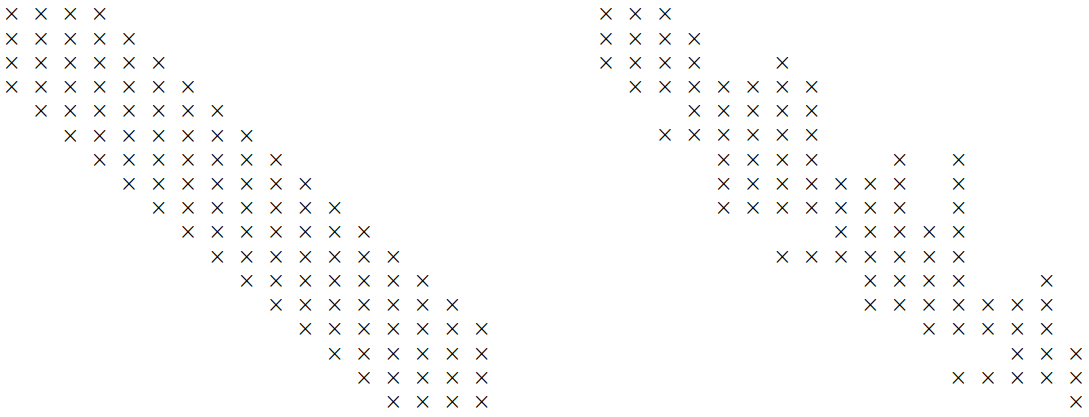
\includegraphics[width=8cm]{png/bandmatrix.png}
    \caption{Band and variable-band matrices.}
    \label{fig:bandedMatrix}
  \end{figure}

  \begin{rmk}
    Finding the banded or variable-band form is based on finding
    permutations to block tridiagonal form. If the blocks are small
    and numerous such a matrix is banded with a small bandwidth.
  \end{rmk}

  \begin{alg}
    The factorization of a block tridiagonal matrix $A$ can be written
    in the form
    $$
    \left[
      \begin{array}{cccccc}
        \mathbf{A}_{11} & \mathbf{A}_{12}& & & & \\
        \mathbf{A}_{21} & \mathbf{A}_{22} & \mathbf{A}_{23} & & &\\
               & \mathbf{A}_{32} & \mathbf{A}_{33} & \cdot & &\\
               & & \cdot & \cdot & \cdot & \\
               & & & \cdot & \cdot & \\
        & & & & \cdot & \mathbf{A}_{NN}
      \end{array}
    \right]=\mathbf{LU},
    $$
    $\mathbf{L}$ and $\mathbf{U}$ can be written in 
    $$
 \mathbf{L}=\left[
      \begin{array}{cccccc}
       \mathbf{I} & & & & & \\
        \mathbf{A}_{21}\mathbf{D}_1^{-1} & \mathbf{I}& & & &\\
               & \ddots & \ddots & & \\
        & &\mathbf{A}_{N,N-1}\mathbf{D}_{N-1}^{-1} & \mathbf{I}
      \end{array}
    \right],
    $$
    $$
    \mathbf{U}=\left[
      \begin{array}{cccccc}
        \mathbf{D}_1 & \mathbf{A}_{12}& & & & \\
         & \mathbf{D}_2& \mathbf{A}_{23}& & &\\
               & & \ddots & \ddots & & \\
               & & & \ddots & \mathbf{A}_{N-1,N} & \\
        & & & & \mathbf{D}_N
      \end{array}
    \right],
    $$
    where
  \begin{align}
    &\mathbf{D}_1=\mathbf{A}_{11},\\
    &\mathbf{D}_i= \mathbf{A}_{ii}-\mathbf{A}_{i,i-1}\mathbf{D}_{i-1}^{-1}\mathbf{A}_{i-1,i},\ i=2,\ldots,N.
  \end{align}
  To use this form to solve a set of equations $\mathbf{Ax=b}$ requires the
  forward substitution steps
  \begin{align}
    &\mathbf{c}_1=\mathbf{b}_1\\
    &\mathbf{c}_i=\mathbf{b}_i-\mathbf{A}_{i,i-1}\mathbf{D}^{-1}_{i-1}\mathbf{c}_{i-1},\ i=2,\ldots,N.
  \end{align}
  followed by the substitution steps
  \begin{align}
   &\mathbf{x}_N=\mathbf{D}^{-1}_N\mathbf{Nc}_N,\\
   &\mathbf{x}_i=\mathbf{D}_i^{-1}\mathbf{c}_i-\mathbf{A}_{i,i+1}\mathbf{c}_{i+1},\ i=N-1,\ldots,1.
  \end{align}
\end{alg} 

\begin{rmk}
   We hope to find an automatic ordering algorithm, such algorithms
   for the symmetric case are the subject of next section.
 \end{rmk}
 
\begin{alg}[Cuthill-McKee algorithm]
  Symmetric permutations of a symmetric matrix correspond to
  relabellings of the nodes of the associated graph and it is easier
  to describe algorithms in terms of relabelling graphs.
  The following is the steps of Cuthill-McKee algorithm:
  \begin{enumerate}[(i)]
  \item Divide the nodes into \emph{level sets}, $S_i$, with
  $S_1$ consisting of a single node. The next, $S_2$, consists of all
  the neighbours of this node. The set $S_3$ consists of all the
  neighbours of the nodes in $S_2$ that are not in $S_1$ or $S_2$. The
  general set $S_i$ consists of lal the neighbours of the nods of
  $S_{i-1}$ that are not in $S_{i-2}$ and $S_{i-1}$.
\item Order within each block $S_i$ by taking first those nodes that
  are neighbours of the first node in $S_{i-1}$, then those that are
  neighbours of the second node in $S_{i-1}$, and so on.
  \end{enumerate}
\end{alg}

\begin{exm}
  The ordering of the Figure \ref{fig:CMcase} could have come from
  level sets (1), (2-4), (5-7), (8-10), (11-13), (14-16), (17) and the
  corresponding matrix shown in Figure \ref{fig:CMcaseMatrix}, is
  block tridiagonal with diagonal blocks having orders 1, 3, 3, 3, 3, 3
  and 1.

  \begin{figure}[H]
    \centering
    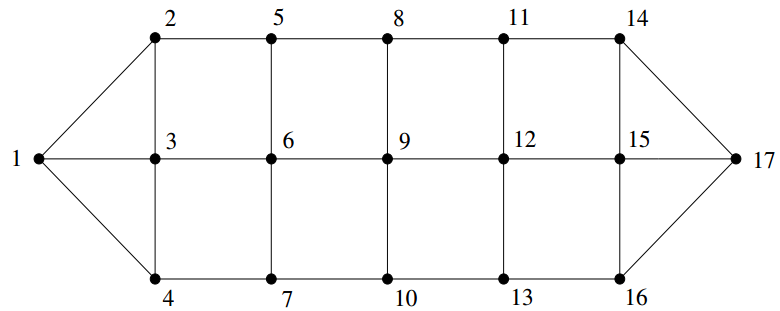
\includegraphics[width=8cm]{png/CMcase.png}
    \caption{A graph with an obviously good node order.}
    \label{fig:CMcase}
  \end{figure}
  \begin{figure}[H]
    \centering
    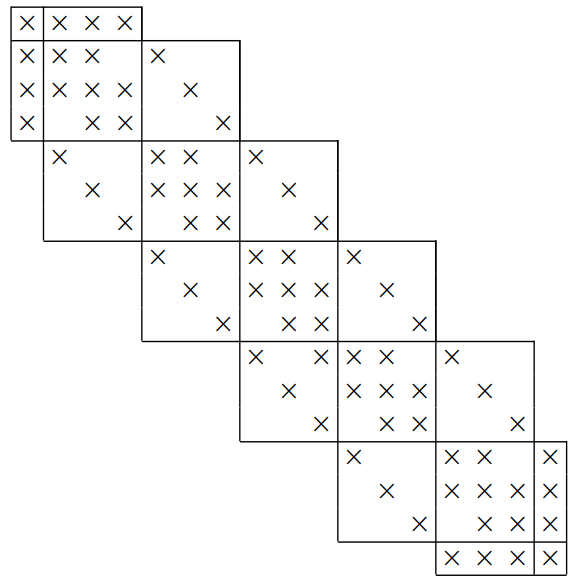
\includegraphics[width=6cm]{png/CMcaseMatrix.png}
    \caption{The matrix corresponding to the Figure \ref{fig:CMcase}
      graph.}
    \label{fig:CMcaseMatrix}
  \end{figure}
\end{exm}

\begin{alg}[the Reverse Cuthill-McKee algorithm(RCM)]
 The only difference with the Cuthill-McKee algorithm is that the
 reverse Cuthill-McKee algorithm orders from the last level set to $S_1$.  
\end{alg}

\begin{rmk}
  Reversing the Cuthill-McKee order often yields a  worthwhile
  improvement, not in the bandwidth, but in the total storage required
  within the variable-band form (the profile) and in the number of
  arithmetic operations required for variable-band factorization. 
\end{rmk}

\begin{exm}
  the Cuthill-McKee order (with level sets (1), (2), (3-7)) is shown
  in Figure \ref{fig:CMorder} and there are 20 zeros within the
  variable-band form. On reversing the order (Figure
  \ref{fig:RCMorder}) all these zeros move outside the form and will
  not need storage. 

  \begin{figure}[H]
    \centering
    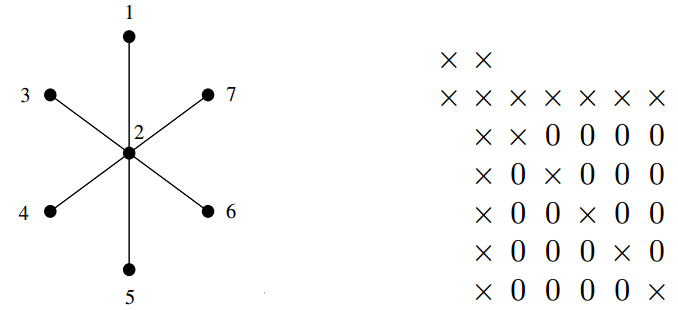
\includegraphics[width=8cm]{png/CMorder.png}
    \caption{A graph and its associated matrix, ordered by Cuthill-McKee.}
    \label{fig:CMorder}
  \end{figure}

  \begin{figure}[H]
    \centering
    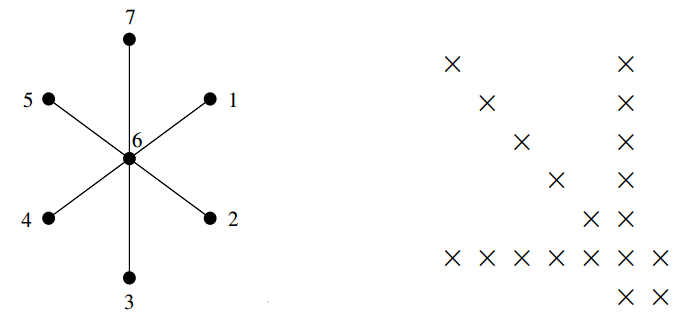
\includegraphics[width=8cm]{png/RCMorder.png}
    \caption{As Figure~\ref{fig:CMorder}, but with order reversed.}
    \label{fig:RCMorder}
  \end{figure}
\end{exm}

\begin{alg}[choosing the starting node for RCM algorithm]
  Each variable in the final level set $S_k$ should be tried as a
  starting node. If one of these nodes produces more than $k$ level
  sets, then this variable replaces the starting node and the new
  level sets are examined, continuing in this way until no further
  increase in the number of level sets is obtained.
\end{alg}

\begin{rmk}
  There are two limitations of the methods of this section:
  \begin{enumerate}
  \item They tend to be less effective when the problems are fully
    two-dimensional, exemplified by a large square grid.
  \item The banded methods are the fundamental sequential nature of
    these orderings. Each computation in the factorization and the
    solve comes from the previous computation. Thus, the methods tend
    to do poorly in a parallel environment.
  \end{enumerate} 
\end{rmk}

\subsection{Orderings based on dissection}
\label{sec:Dissection}

\begin{defn}
  There are two desirable form: \emph{bordered block diagonal form} and
  \emph{doubly-bordered block diagonal form}, which are illustrated in Figure \ref{fig:BBTF}
  and Figure \ref{fig:DBBTF}.

  \begin{figure}[H]
    \centering
    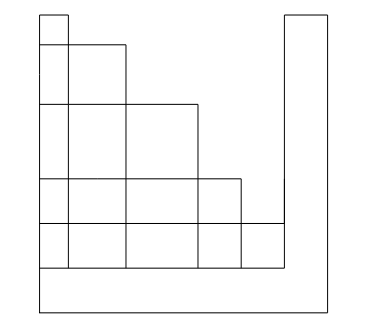
\includegraphics[width=4cm]{png/BorderedBlockDF.png}
    \caption{Bordered block triangular form.}
    \label{fig:BBTF}
  \end{figure}
  \begin{figure}[H]
    \centering
    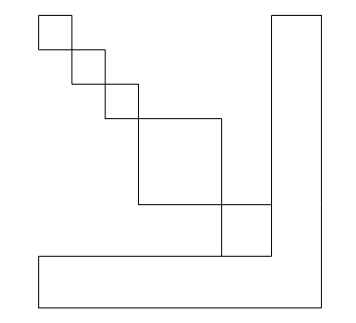
\includegraphics[width=4cm]{png/DBorderedBlockDF.png}
    \caption{Doubly-bordered block triangular form.}
    \label{fig:DBBTF}
  \end{figure}
  
\end{defn}
\begin{exm}
  To establish the basic idea, consider the graph in Figure
  \ref{fig:onewayDissectionCase} with the
  columns in the order $(1,2,4,5,7,8,10,11,3,6,9).$ A way to motivate
  this ordering is to look at the entire graph, and select nodes
  which, when removed, dissect the graph into smaller pieces. The
  effect of this ordering can be seen in the matrix pattern in
  Figure \ref{fig:onewayDissectionCaseMatrix}. We make two observations about this matrix pattern:
  \begin{enumerate}
  \item The ordering leads to a matrix that has a bordered block diagonal
form with four diagonal blocks. Fill-in is confined to the diagonal
blocks and the borders.
\item Factorization of the first four diagonal blocks can be performed independently,
allowing an easy exploitation of parallelism.
\end{enumerate}

\begin{figure}[H]
  \centering
  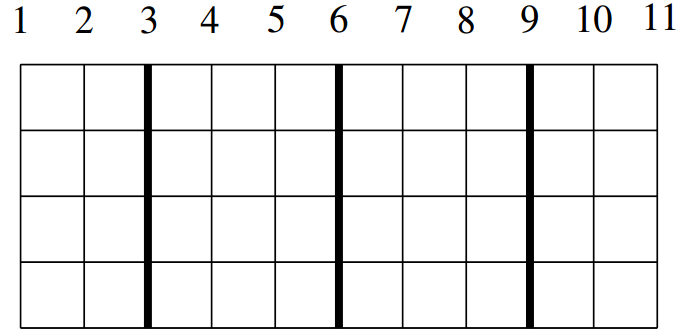
\includegraphics[width=7cm]{png/onewayDissectionCase.png}
  \caption{A regular $5\times 11$ grid problem, one-way dissected.}
  \label{fig:onewayDissectionCase}
\end{figure}
\begin{figure}[H]
  \centering
  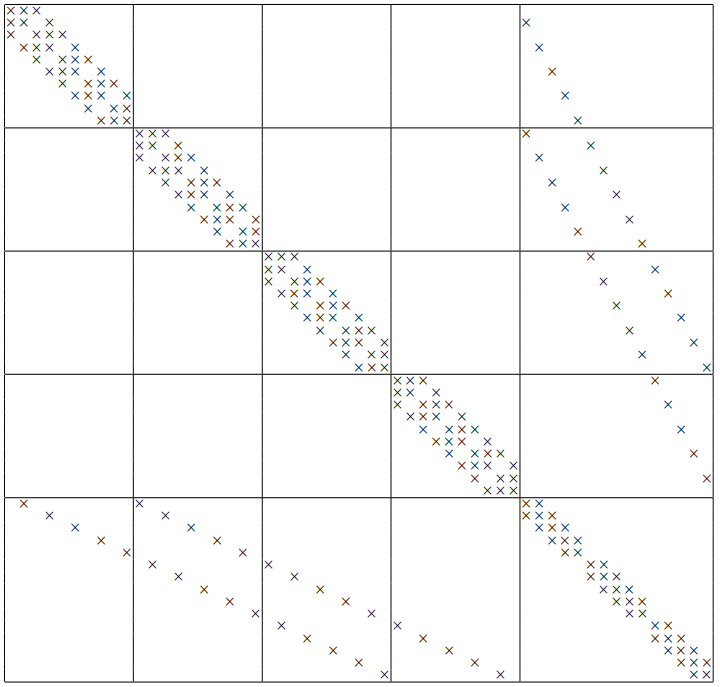
\includegraphics[width=8cm]{png/onewayDissectionMatrix.png}
  \caption{The matrix arising from one-way dissection of the problem
    in Figure \ref{fig:onewayDissectionCase}.}
  \label{fig:onewayDissectionCaseMatrix}
\end{figure}
\end{exm}

\begin{alg}
  Similarly to the way we dealt with the block tridiagonal forms in
  Section \ref{sec:BandSolution}, The factorization of a
  doubly-bordered block tridiagonal matrix $\mathbf{A}$ can be written
    in the form
    $$
    \left[
      \begin{array}{ccccc}
        \mathbf{A}_{11} & & & & \mathbf{A}_{1N} \\
        & \mathbf{A}_{22} & & & \mathbf{A}_{2N}\\
               & & \mathbf{A}_{33} & & \mathbf{A}_{3N}\\
            &   & & \ddots & \vdots  \\
        \mathbf{A}_{N1}& \mathbf{A}_{N2}& \mathbf{A}_{N3}& \cdots & \mathbf{A}_{NN}
      \end{array}
    \right]=\mathbf{LU},
    $$
    $\mathbf{L}$ and $\mathbf{U}$ can be written in 
    $$
 \mathbf{L}=\left[
      \begin{array}{ccccc}
        \mathbf{I} & & & &  \\
        & \mathbf{I}& & & \\
               & & \mathbf{I}& & \\
               & & & \ddots&  \\
        \mathbf{A}_{N1}\mathbf{D}_1^{-1}& \mathbf{A}_{N2}\mathbf{D}_2^{-1}& \mathbf{A}_{N3}\mathbf{D}_3^{-1}& \cdots & \mathbf{I}
      \end{array}
    \right],
    $$
    $$
    \mathbf{U}=\left[
      \begin{array}{ccccc}
        \mathbf{D}_1 & & & & \mathbf{A}_{1N} \\
         & \mathbf{D}_2& & & \mathbf{A}_{2N}\\
               & & \mathbf{D}_3& & \mathbf{A}_{3N}\\
               & & & \ddots& \vdots \\
        & & & & \mathbf{D}_N
      \end{array}
    \right],
    $$
    where
  \begin{align}
    &\mathbf{D}_i=\mathbf{A}_{ii},\ i=1,2,\ldots,N-1.\\
    &\mathbf{D}_N= \mathbf{A}_{NN}-\sum\limits_{j=1}^{N-1}\mathbf{A}_{Nj}\mathbf{D}_{j}^{-1}\mathbf{A}_{jN}.
  \end{align}
  To use this form to solve a set of equations $\mathbf{Ax=b}$ , we can carry
  out the solution in the following way:
  \begin{align}
    &\mathbf{c}_i=\mathbf{b}_i,\ i=1,2,\ldots,N-1\\
    &\mathbf{c}_N=\mathbf{b}_N-\sum\limits_{j=1}^{N-1}\mathbf{A}_{Nj}\mathbf{D}^{-1}_{j}\mathbf{c}_{j},
  \end{align}
  followed by the substitution steps
  \begin{align}
   &\mathbf{x}_N=\mathbf{D}^{-1}_N\mathbf{c}_N,\\
   &\mathbf{x}_i=\mathbf{D}_i^{-1}(\mathbf{c}_i-\mathbf{A}_{iN}\mathbf{c}_{N}),\ i=N-1,\ldots,1.
  \end{align}
\end{alg}

\begin{alg}[Finding the dissection cuts for one-way dissection]
  For automatic one-way dissection of a general problem, George (1980)
  proposed the algorithm for finding the dissection cuts:
  \begin{enumerate}[(i)]
  \item  Firstly, generate a good level structure, as in Section \ref{sec:BandSolution}.
  \item Compute the average number of nods at each level, say $m$.
  \item Take points from each of the level sets $S_j$ where
    \begin{equation}
      \label{eq:DissectionCutsLevelSet}
      j=\lfloor i\delta+0.5\rfloor,\ i=1,2,\ldots
    \end{equation}with spacing
    \begin{equation}
      \label{eq:DissectionCutsSpacing}
      \delta=\sqrt{\frac{3m+13}{2}}.
    \end{equation}
  \end{enumerate}
  The formula \eqref{eq:DissectionCutsSpacing} for the spacing was
  chosen by George on the basis of numerical experiments and analysis
  of regular grids, with the aim of keeping storage requirements
  low. It would suffice to place all the points in the level sets
  \eqref{eq:DissectionCutsLevelSet} in the last block and the points
  in the intervening groups of level sets into the other blocks.
\end{alg}

\begin{defn}
  The \emph{row graph} of a matrix $A$ is the graph with vertices that
  correspond to the rows of $A$ and with an edge between two vertices
  if and only if there is at least one column that has an entry in
  both of the corresponding rows.
\end{defn}

\begin{exm}
  There is an example of a matrix and its row graph in Figure \ref{fig:RowGraph}.
  \begin{figure}[H]
    \centering
    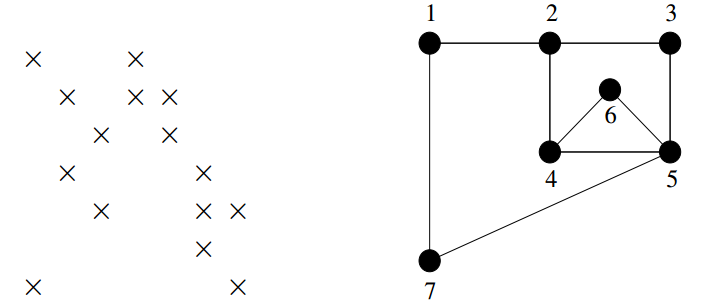
\includegraphics[width=7cm]{png/RowGraph.png}
    \caption{A matrix and its associated row graph.}
    \label{fig:RowGraph}
  \end{figure}
\end{exm}
 
\begin{prop}
  The graph of $\mathbf{AA^T}$ is the row graph of $\mathbf{A}$.
\end{prop}

\begin{defn}
  A \emph{hypergraph} is a generalization of a graph in which an edge can
  join any number of vertices. The generalized edges are called
  \emph{nets} (also known as \emph{hyperedges}). The vertices in a net
  are called its \emph{pins} and \emph{the size of a net} is its
  number of pins. \emph{The degree of a vertex} is the number of nets in
  which it is a pin. Vertex $i$ can have an associated \emph{weight} $w_i$
  and net $i$ can have an associated \emph{cost} $c_i$.
\end{defn}

\begin{defn}
  In a partition, the set of vertices (rows) is divided into $k$
  distinct non-empty \emph{parts} and a net (column) is regarded as being
  \emph{connected} to a part if it has at least one pin in the part.
\end{defn}

\begin{thm}
  By permuting the vertices so that those in each part are together
  and permuting the nets so that those with pins only in part 1 come
  first, then those with pins only in part 2, and then those with pins
  only in part $k$, and finally those with pins in more than one part,
  we obtain the singly bordered block diagonal form illustrated in
  Figure \ref{fig:SinglyBBDF}. 
  \begin{figure}[H]
    \centering
    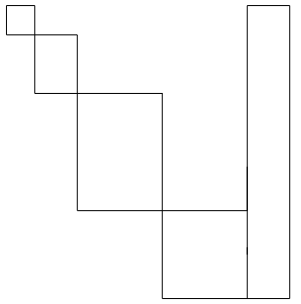
\includegraphics[width=4cm]{png/SinglyBBDF.png}
    \caption{A singly bordered block diagonal form.}
    \label{fig:SinglyBBDF}
  \end{figure}
\end{thm}

\begin{defn}
  The \emph{connectivity} of net (column) $i$, denoted by $\lambda_i$,
  is defined as the number of parts to which it is connected. It is
  said to be \emph{cut} (or \emph{external}) if $\lambda_i>1$. It is the cut nets
  that we permute to the border.
\end{defn}

\begin{defn}
  A partition has an associated \emph{cost}. The two most common are
  the sum of the costs $c_i$ of the cut nets and the sum of the
  weighted sums $c_i(\lambda_i-1)$ of the cut nets. 
\end{defn}

\begin{prop}
  With $c_i=1$, the first cost is the number of columns in the border
  and the second cost corresponds to the amount of communication for
  distributed matrix-vector multiplication.
\end{prop}

\begin{rmk}
  As in the case of graphs, a good partitioning should minimize the
  cost while maintaining a balance between the parts. If the weight
  $W_i$ of part $i$ is defined as the sum of the weights $w_i$ of the
  vertices (rows) in it, a common \emph{balance criterion} is to
  require
  \begin{equation}
    \label{eq:BalanceCriterion}
    W_i\leq W_{avg}(1+e),\ \forall i=1,\ldots,k
  \end{equation}
  where $W_{avg}$ is the average weight of a part and $e$ is a
  tolerance on balance, typically between 0.25 and 1.0.
\end{rmk}

\begin{rmk}
  We seek to partition the rows into two sets such that only a few
  columns have entries in both sets.
\end{rmk}

\begin{defn}
  The \emph{net-cut} is defined as the number of columns with entries
  in both partitions and will be equal to the number of border columns
  in the reordered form.
\end{defn}

\begin{defn}
  A \emph{boundry row} is a row in one set of the current partition
  that is connected in the row graph to a row in the other set of the
  partition (has an entry in the same column as a row of the other
  partition).
\end{defn}

\begin{defn}
  For each row, we can compute the change in the net-cut value caused
  if the row were moved to the other partition. This is called the \emph{gain}.
\end{defn}

\begin{alg}
  The algorithm is used to improve a given partition:
\begin{figure}[H]
    \centering
    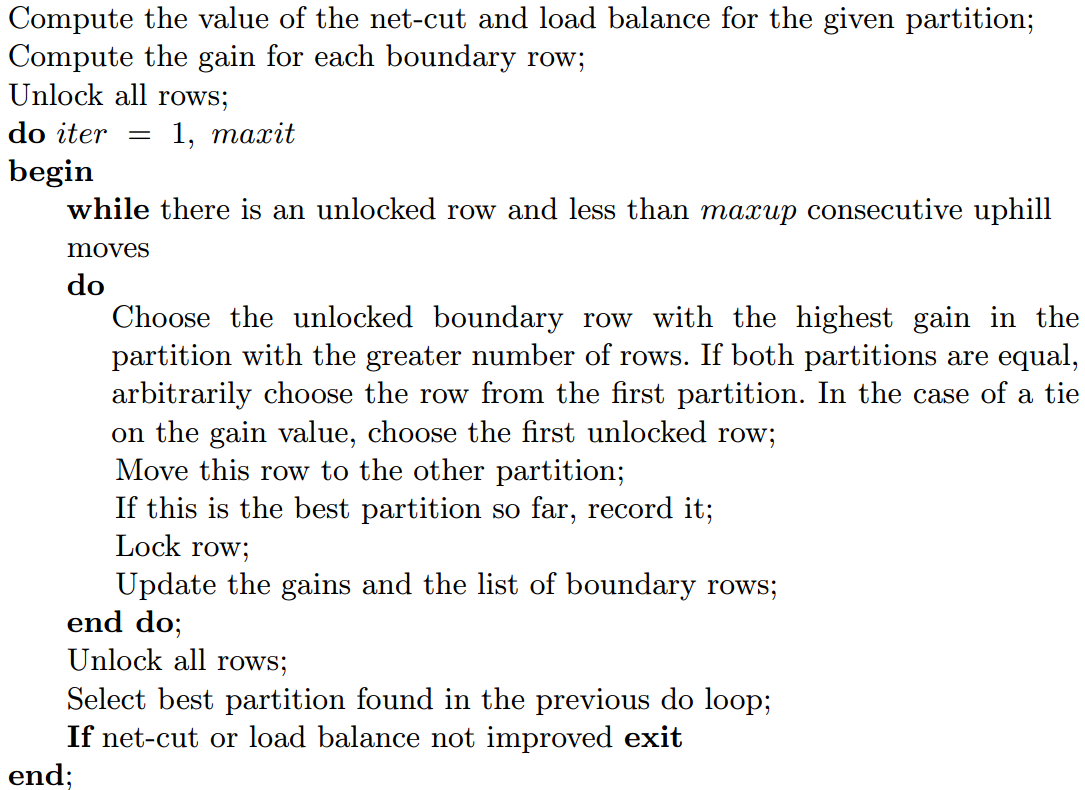
\includegraphics[width=9cm]{png/LinAlgorithm.png}
    \caption{A summary of the Kernighan and Lin (1970) algorithm in
      pseudo-algol.}
    \label{fig:LinAlgorithm}
  \end{figure}
\end{alg}

\begin{rmk}
  To find an appropriate starting point for the Kernighan and Lin
  algorithm, we would use this algorithm wihin a multilevel
  scheme. The strategy is coarsening algorithm to coarsen the matrix recursively
  and then applies the Kernighan and Lin algorithm to the graph of
  each level.
\end{rmk}

\begin{alg}
  The strategy used by \texttt{MONET} algorithm for coarsening the pattern of
  the unsymmetric matrix is to recognize and combine pairs of rows
  that have similar patterns. The algorithm for doing this is given in
  Figure \ref{fig:Monet}. 

  \begin{figure}[H]
    \centering
    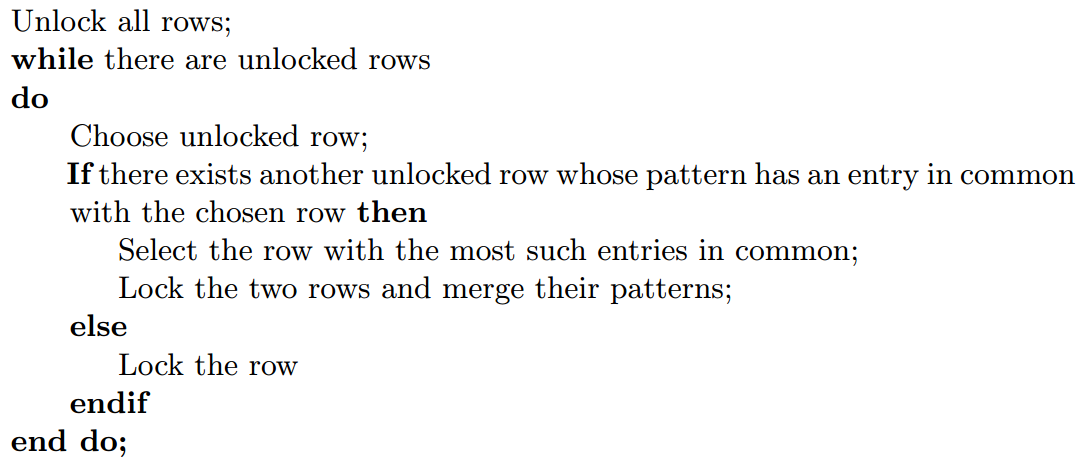
\includegraphics[width=9cm]{png/MONET.png}
    \caption{A summary of the \texttt{MONET} coarsening algorithm in
      pseudo-algol.}
    \label{fig:Monet}
  \end{figure}

  This coarsening is continued until the number of rows in the coarse matrix is
less than a preset number (default 100 in \texttt{HSL\_MC66}) or the ratio of the number
of rows in consecutive matrices is more than a preset fraction (default 0.75 in
\texttt{HSL\_MC66}).
\end{alg}

\begin{rmk}
  The \texttt{MONET} approach coarsens the matrix recursively and then applies
the Kernighan and Lin algorithm to the graph
corresponding to the coarsest matrix from an arbitrary starting partition with
roughly equal numbers of rows in its two sets and with its parameters set very
high in the hope of getting a near optimal partition on this small
matrix.

This partition is then prolongated to the next finer graph through expanding the
rows that were collapsed in that level of the coarsening. The Kernighan and Lin
algorithm is then applied with this partition as the starting point
and the process is repeated up to the finest graph corresponding to the original
matrix. The columns of the net-cut are moved to the border.
\end{rmk}
%%% Local Variables:
%%% mode: latex 
%%% TeX-master: "LU_MathDocument"
%%% End:


\section{Gilbert's LU factorization for sparse matrix}
This section is based on \cite{Gilbert1988}.

\begin{defn}[Symbolic analysis]
    When solving problems for sparse matrix, it's usually 
    more efficient when working with a fixed datastructure. 
    \textit{Symbolic analysis} is such a precursor to the 
    numerical solution, it includes computations that 
    typically depend only on the nonzero pattern, not the 
    numerical values. This will give a nonzero pattern of the 
    solution, so we can use a fixed datastructure to 
    store it.
\end{defn}

\begin{defn}
    Graph theory is a fundamental tool in sparse matrix 
    techniques. Graph $G_\mA=(V,E)$ for an 
    $\mathbb{R}^{n\times n}$ sparse matrix $\mA$ is defined by 
    vertices $V=\{1,\ldots,n\}$, edges $E=\{i\rightarrow j:
    a_{ij}\neq 0\}$ or $E=\{i\rightarrow j:a_{ji}\neq 0\}$ which 
    depend on the problem. When the matrix is symmetric, the 
    graph can be undirected. 
\end{defn}

\subsection{Solution for sparse triangular systems}
\label{section::sparseLxb}
\begin{lem}
    \label{lem::dfs}
    When we solve $\mL\mx=\mathbf{b}$, where both $\mL$ and 
    $\mathbf{b}$ are sparse and $\mL$ is lower triangular, 
    we should first use symbolic analysis to find the nonzero 
    pattern of $\mx$. This can be done by a depth-first search 
    in $G_\mL$ start with $\{i:b_i\neq 0\}$ where 
    $E=\{i\rightarrow j:l_{ji}\neq 0\}$. 
\end{lem}
\begin{proof}
    Formally, we have the relation
    \begin{equation}
        \label{eq::xiequation}
        x_i=b_i-\sum_{j=1}^{i-1}l_{ij}x_j.
    \end{equation}
    Notice that we are doing symbolic analysis, so we assume 
    no zero is produced during numerical calculation. So 
    $b_i\neq 0$ or $x_j\neq 0\cap l_{ij}\neq 0$ means there is 
    at least one nonzero term in \eqref{eq::xiequation}, so 
    \begin{align*}
        &b_{i}\neq 0\Rightarrow x_i\neq 0,\\
        &x_j\neq 0\cap l_{ij}\neq 0\Rightarrow x_i\neq 0.
    \end{align*}

    Now, assume $b_i\neq 0$, then $x_i\neq 0$. For all 
    $\{j:l_{ji}\neq 0\}$, we have $x_j\neq 0$, which is 
    equivalent to find all nodes who has an edge start from 
    $i$. Continue this search so we can find all $x_k\neq 0$ 
    because $b_i\neq 0$, this is indeed a search in 
    $G_\mL$. Do this for all $\{i:b_i\neq 0\}$, then we 
    find the nonzero pattern of $\mx$. Usually, the search is 
    performed by depth-first search.
\end{proof}

\begin{exm}
    For example, when we have $\mL$ and $G_\mL$ as in Figure 
    \ref{fig::LGL}.
    \begin{figure}[H]
        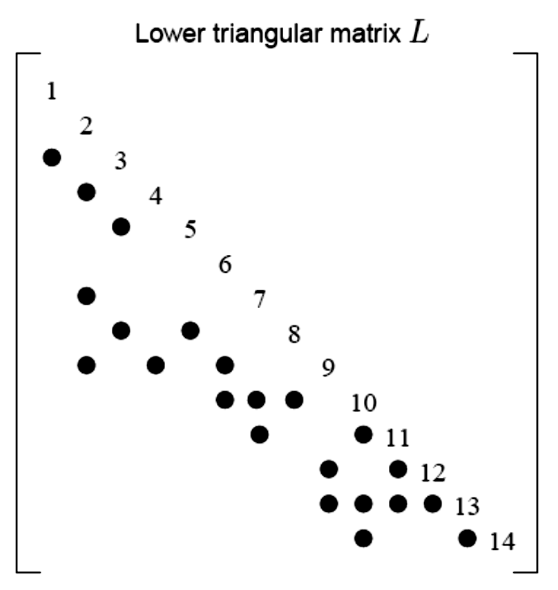
\includegraphics[width=0.49\linewidth]{png/L.png}
        \hfill
        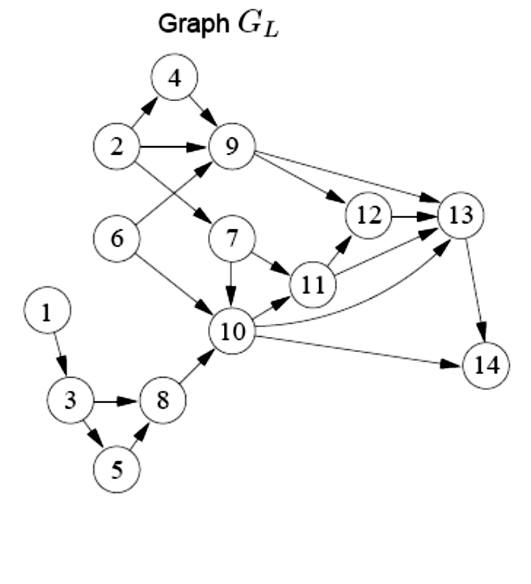
\includegraphics[width=0.49\linewidth]{png/GL.png}
        \caption{$\mL$ and corresponding $G_\mL$}
        \label{fig::LGL}
    \end{figure}
    Assuming only $b_4,b_6\neq 0$, then the depth-first 
    search paths are as in Figure \ref{fig::LGL2}, where the 
    red points in $\mL$ represent the edges in the search 
    paths.
    \begin{figure}[H]
        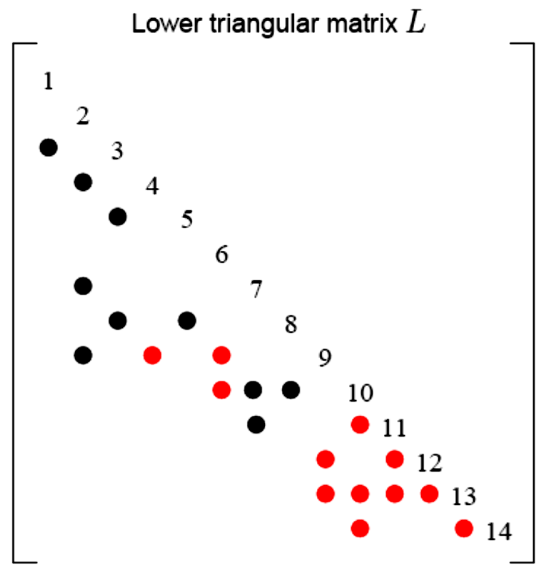
\includegraphics[width=0.49\linewidth]{png/L2.png}
        \hfill
        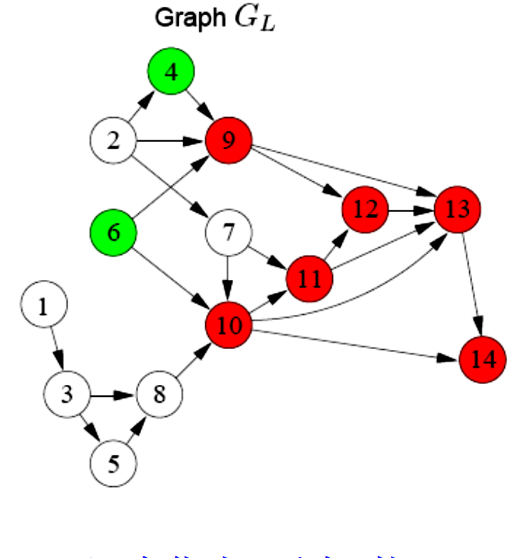
\includegraphics[width=0.49\linewidth]{png/GL2.png}
        \caption{The search paths of $\mL\mx=\mathbf{b}$}
        \label{fig::LGL2}
    \end{figure}
\end{exm}

\begin{lem}
    \label{lem::toporder}
    When we solve $\mL\mx=\mathbf{b}$ where $\mL$ is dense, we 
    use forward substitution, which would solve for the 
    unknowns in increasing order of row number. However, the 
    depth-first search may not find the nonzero positions of 
    $x_j$ in this order, and we don't want to sort it because 
    even a bucket sort would take $\mathcal{O}(n)$ time. 

    The solution to this problem is adding a stack during the 
    depth-first search, each time the depth-first search 
    backtracks from a vertex, that vertex is pushed into the 
    stack. After all the searches are done, the reverse order 
    of the stack is thus the order which will be used in 
    solving $x_j$, this order is also called the \textit{
    topological order}.
\end{lem}
\begin{proof}
    By \eqref{eq::xiequation}, we know that $x_i$ can be 
    calculated as soon as all the $\{x_k:l_{ik}\neq 0\cap 
    x_k\neq 0\}$ have been calculated. Notice that in the 
    depth-first search, if $l_{ik}\neq 0\cap x_k\neq 0$, 
    there must be an edge $k\rightarrow i$ in the search paths. 
    So, when the depth-first search backtracks from $i$, all 
    $\{k:l_{ik}\neq 0\cap x_k\neq 0\}$ are not in the stack 
    yet, otherwise there will be a contradiction. So when we 
    solve $x_i$ in the reverse order of the stack, we will 
    calculate all $\{x_k:l_{ij}\neq 0\cap x_k\neq 0\}$ before 
    we calculate $x_i$.
\end{proof}

\begin{thm}
    \label{thm::sparseLxbcost}
    The sparse lower triangular systems $\mL\mx=\mathbf{b}$ can 
    be solved in $\mathcal{O}(\mathrm{flops}(\mL\mx)+
    \eta(\mathbf{b}))$ time, where $\mathrm{flops}(\mL\mx)$ is 
    the number of multiplications of nonzeros when calculating 
    $\mL\mx$, $\eta(\mathbf{b})$ is the number of nonzeros in 
    $\mathbf{b}$.
\end{thm}
\begin{proof}
    There are two stages in solution, the depth-first search and 
    numerical calculation. The depth-first search takes time 
    proportional to the number of starting vertices plus the 
    number of edges traversed. The number of starting vertices 
    is obviously $\eta(\mathbf{b})$. The number of edges 
    traversed is the number of $\{(i,j):x_i\neq 0\cap 
    l_{ji}\neq 0\}$, notice that $(\mL\mx)_j=
    \sum_{\{i:x_i\neq 0\cap l_{ji}\neq 0\}}l_{ji}x_i$, so the 
    number of edges is exactly $\mathrm{flops}(\mL\mx)$. 

    As for the numerical calculation stage, since we know the 
    nonzero structure of $\mx$ before we start, we need only 
    initialize and manipulate the positions in the dense 
    vector that corresponding to nonzero positions, thus the 
    whole thing still takes only $\mathcal{O}(\mathrm{flops}
    (\mL\mx)+\eta(\mathbf{b}))$ time.
\end{proof}

\subsection{LU factorization with partial pivoting for sparse 
matrix}
\begin{alg}
    \label{alg::sparseLU}
    Since partial pivoting is used, we can't predict the 
    nonzero structure of the whole factors. \cite{Gilbert1988} 
    then compute the factors column by column just like the 
    left-looking LU factorization. Additionally, the 
    computation of each column of the factors is breaked into a 
    symbolic and numerical stage. Recall the procedure of 
    left-looking LU factorization with partial pivoting.
    \IncMargin{1em}
    %\LinesNumbered
    \begin{algorithm}[H]
        \caption{Left-looking LU factorization with partial 
        pivoting}
        \SetKwInOut{Precond}{Preconditions}
        \SetKwInOut{Postcond}{Postconditions}

        \KwIn{$\mA\in\mathbb{R}^{n\times n}$}
        \Precond{$\mA$ is nonsingular}
        \KwOut{$\mL,\mU\in\mathbb{R}^{n\times n}$}
        \Postcond{$\mL$ is unit lower triangular, $\mU$ is 
        upper triangular}

        \BlankLine
        $\mathbf{b}(1:n)=0$\;
        \For{$j=1:n$}{
            Solve $\mL(1:(j-1),1:(j-1))\mU(1:(j-1),j)=
            \mA(1:(j-1),j)$\;
            $\mathbf{b}(j:n)=\mA(j:n,j)-\mL(j:n,1:(j-1))
            \mU(1:(j-1),j)$\;
            Pivot: swap $b_{j}$ with the largest-magnitude 
            element of $\mathbf{b}(j:n)$, swap $\mL$ and $\mA$\;
            $u_{jj}=b_{j}$\;
            $\mL(j:n,j)=\mathbf{b}(j:n)/u_{jj}$\;
        }
    \end{algorithm}
    \DecMargin{1em}
    The left-looking LU factorization with partial pivoting 
    for sparse matrix is actually in the same form, excluding 
    the way to solve $\mL(1:(j-1),1:(j-1))\mU(1:(j-1),j)=
    \mA(1:(j-1),j)$. For sparse matrix, this lower triangular 
    systems can be solved just like what we have discussed in 
    Section \ref{section::sparseLxb}.
\end{alg}

\begin{thm}
    The entire algorithm \ref{alg::sparseLU} can be implmented 
    to run in $\mathcal{O}(\mathrm{flops}(\mL\mU)+\eta(\mA))$.
\end{thm}
\begin{proof}
    Define $m=\eta(\mA),\,m^*=\eta(\mL-\mI+\mU)$, then one can 
    show that $m^*-m\leq \mathrm{flops}(\mL\mU)$ because any 
    created nonzero element in $\mL-\mI+\mU$ is used in 
    $\mL\mU$ to balance other terms to make $\mL\mU=\mA$ hold. 
    
    By Theorem \ref{thm::sparseLxbcost}, step 2 and step 3 in 
    algorithm \ref{alg::sparseLU} take total time $\mathcal{O}
    (\mathrm{flops}(\mL\mU)+m^*)$ plus $\mathcal{O}(n)$ to 
    initialize the mark array for the depth-first search. Step 
    4 and step 6 each examine every nonzero in $\mL$ once, so 
    they take time $\mathcal{O}(m^*)$ over all. Step 5 takes 
    $\mathcal{O}(n)$ time overall. Since $n\leq m\leq m^*\leq 
    \mathrm{flops}(\mL\mU)+m$, the total is $\mathcal{O}
    (\mathrm{flops}(\mL\mU)+\eta(\mA))$.
\end{proof}

\section{Frontal method}
\subsection{Introduction}
\begin{exm}
    In the methods for factorization discussed earlier in this 
    chapter, we have assumed that the matrix $\mA$ is given. 
    However, the matrix is `assembled' as the sum of 
    submatrices sometimes, mostly in finite-element problems. 

    In a finite-element problem the matrix is a sum
    \begin{equation}
        \label{eq::assemble}
        \mA=\sum_l\mA^{[l]},
    \end{equation}
    where each $\mA^{[l]}$ has entries only in the principal 
    submatrix corresponding to the variables in element $l$ 
    and represents the contributions from this element. It is 
    normal to hold each $\mA^{[l]}$ in packed form as a small 
    full matrix together with a list of indices of the 
    variables that are associated with element $l$.
\end{exm}

\begin{defn}[Fully summed]
    The formation of the sum \eqref{eq::assemble} is called 
    \textit{assembly} and involves the elementary operation
    \begin{equation}
        \label{eq::elementassemble}
        a_{ij}:=a_{ij}+a_{ij}^{[l]}.
    \end{equation}
    We have used the Algol symbol ‘$:=$’ here to avoid 
    confusion with the superscript notation $a_{ij}^{(k)}$. 
    We call an entry \textit{fully summed} when all 
    contributions of the form \eqref{eq::elementassemble} have 
    been summed.
\end{defn}

\begin{lem}
    \label{lem::frontaleliminate}
    It is evident that basic operation of Gaussian elimination
    \begin{equation}
        \label{eq::frontaleliminate}
        a_{ij}^{(k+1)}=a_{ij}^{(k)}-a_{ik}^{(k)}(a_{kk}^{(k)})^
        {-1}a_{kj}^{(k)}
    \end{equation}
    may be performed before all the assemblies 
    \eqref{eq::elementassemble} are complete, provided only the 
    terms in the triple product in \eqref{eq::frontaleliminate} 
    are fully summed. Each variable can be eliminated as soon 
    as its row and column is fully summed, that is after its 
    last occurrence in a matrix $\mA^{[l]}$.
\end{lem}

\begin{defn}
    By Lemma \ref{lem::frontaleliminate}, the elimination 
    operations will be confined to the submatrix of rows and 
    columns corresponding to variables that have not yet been 
    eliminated, but are involved in one or more of the elements 
    that have been assembled. This permits all intermediate
    working to be performed in a full matrix whose size 
    increases when a variable appears for the first time and 
    decreases when one is eliminated. The pivotal order is 
    determined from the order of the assembly. If the elements 
    are ordered systematically from one end of the region to 
    the other, the active variables form a front that moves 
    along it. For this reason, the full matrix in which all 
    arithmetic is performed is called the \textit{frontal 
    matrix} and the technique is called the 
    \textit{frontal method}.
\end{defn}

\begin{exm}
    In Figure \ref{fig::Frontal}, we show the situation after 
    a set of elimination and just prior to another assembly. 
    The fully-summed rows and columns in blocks $(1,1)$, 
    $(1,2)$ and $(2,1)$ contain the corresponding rows and 
    columns of $\mL$ and $\mU$. They will not be needed until 
    the solve stage, so may be stored on auxiliary storage as
    packed vectors. Blocks $(3,1)$ and $(1,3)$ are zero 
    because the eliminated variables are fully summed. Block 
    $(2,2)$ is the frontal matrix, normally held in memory. 
    Blocks $(2,3)$, $(3,2)$, and $(3,3)$ as yet have no 
    contributions, so require no storage.
    \begin{figure}[H]
        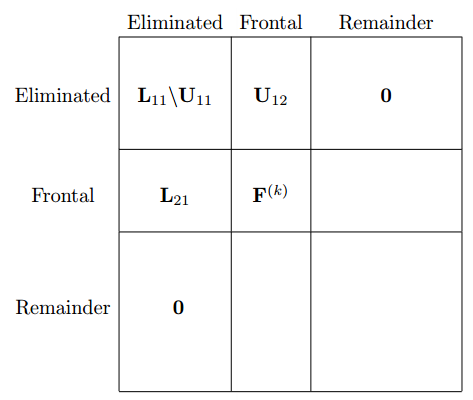
\includegraphics[width=0.8\linewidth]{png/Frontal.png}
        \caption{Matrix of partially processed frontal method}
        \label{fig::Frontal}
    \end{figure}
\end{exm}

\subsection{Element assembly tree}
In this section, we assume that the assembled matrix is 
SPD so that numerical pivoting is not 
needed for stability.
\begin{defn}
    Consider the finite-element case. The grouping of elements 
    into substructures and of substructures into bigger 
    substructures until the whole problem is obtained can be 
    expressed as a tree that is know as an \textit{element 
    assembly tree}. In an element assembly tree, each node 
    corresponds to an assembly of a frontal matrix (nothing to 
    do at a leaf node) and subsequent eliminations to form the 
    generated element matrix (also known as the `contribution 
    block').
\end{defn}

\begin{exm}
    For the finite-element problem shown on the left of Figure 
    \ref{fig::FEMproblem}, the substructure defined by nested 
    dissection can be represented by the tree shown on the 
    right of Figure \ref{fig::FEMproblem}
    \begin{figure}[H]
        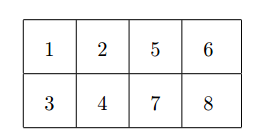
\includegraphics[width=0.45\linewidth]{png/FEMproblem.png}
        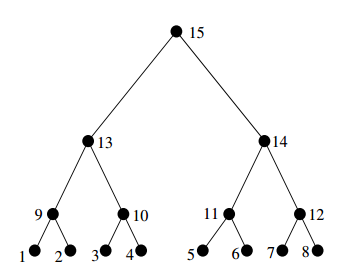
\includegraphics[width=0.45\linewidth]{png/assemblytree.png}
        \caption{A finite-element problem and the corresponding 
        element assembly tree}
        \label{fig::FEMproblem}
    \end{figure}
    This nested grouping of elements into substructures can 
    also be represented by bracketing of the sum
    \begin{align*}
        \mA=\sum_{l}\mA^{[l]}=&((\mA^{[1]}+\mA^{[2]})+
        (\mA^{[3]}+\mA^{[4]})+\\
        &(\mA^{[5]}+\mA^{[6]})+(\mA^{[7]}+\mA^{[8]})).
    \end{align*}
    For the above element assembly tree, we may perform the 
    eliminations as follows:
    \begin{enumerate}[(i)]
        \item Eliminate all variables that belong in only one 
                element, storing the resulting pivotal rows 
                and columns, and setting the resulting 
                generated element matrices aside temporarily.
        \item Assemble the resulting matrices in pairs and  
                eliminate any variable that is internal to a 
                single pair; store the resulting generated element matrices $\mA^{[9]}\sim\mA^{[12]}$.
        \item Repeat the second step until there is only one 
                structure.
    \end{enumerate}
\end{exm}

\subsection{Elimination tree}
In this section, we take as our starting point a given 
SPD matrix of order $n$.

\begin{defn}
    Just like the element assembly tree, we can construct a 
    tree called \textit{elimination tree} to arrange the 
    ordering of the elimination. It has a node for each row of 
    the matrix, if node $a$ is a child of node $b$, it means 
    that the elimination of pivot $a$ will have contribution 
    to $b$.
\end{defn}

\begin{lem}
    \label{lem::emtree}
    Suppose row $k$ has the first off-diagonal entry in the 
    column $l>k$, then row $k$ must appear ahead of row $l$ 
    since otherwise the numerical values in row $l$ when it 
    becomes pivotal will be different. We represent this by an 
    edge $(k,l)$. For any other entry $m>l$, the elimination 
    at step $k$ will fill entry $a_{lm}^{(k)}$, if not already 
    filled, so $m$ must be an ancestor of $l$ (when $m$ is 
    smaller than the first off-diagonal entry in row $l$ when 
    eliminating pivot $l$, $m$ will be the parent of $l$). By 
    this procedure, for any node $k_1$, we can get a sequence 
    of edges to nodes $k_1<k_2<...<k_r$, ending at a node 
    $k_r$ corresponding to a row that has no entries to the 
    right of the diagonal when eliminating it.
\end{lem}

\begin{exm}
    In Figure \ref{fig::emtree}, row $1$ and $2$ may be 
    interchanged without having any effect on the operations 
    performed, but row $1$ must precede row $3$. Since $3$ is 
    the first off-diagonal entry when eliminating pivot $1$, 
    it will be the parent of $1$. Since $a_{24},a_{25}\neq 0$, 
    there will be a fill-in in position $a_{45}^{(2)}$, so row 
    $4$ must precede row $5$. Since $5$ is the first 
    off-diagonal entry when eliminating pivot $4$, it will be 
    the parent of $4$. The corresponding elimination tree is 
    shown on the right of Figure \ref{fig::emtree}.
    \begin{figure}[H]
        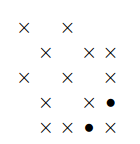
\includegraphics[width=0.45\linewidth]{png/emtree1.png}
        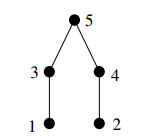
\includegraphics[width=0.45\linewidth]{png/emtree2.png}
        \caption{A matrix (each fill-in is marked as a point) 
        and the corresponding elimination 
        tree}
        \label{fig::emtree}
    \end{figure}
\end{exm}

\begin{alg}[Generate the elimination tree]
    \label{alg::emtree}
    \cite{Liu1986} has given an efficient way to generate the 
    elimination tree, essentially in time proportional to the 
    number of entries in the original matrix.

    We first consider what happens if we try to generate the
    elimination tree for a symmetric matrix that is reducible, 
    that is, a permutation of a block diagonal matrix. The 
    equations for a single block are then independent of the 
    other equations and the elimination tree for this block 
    will have as its root the node corresponding to the 
    variable in the block that is last in the pivotal order. If 
    there are $m$ blocks, there will be $m$ such elimination 
    trees, so we have a forest. So now we only consider 
    irreducible matrices.

    The $k$-th stage ($k=1,...n$) of Liu's algorithm starts 
    with the elimination forest for the leading submatrix of 
    order $k-1$, this will often be a forest rather than a tree 
    since a submatrix of an irreducible matrix may be 
    reducible. He then add the entries of column $k$ of the 
    original matrix one by one and the forest is updated to 
    correspond. He starts by adding a one node for column $k$. 
    When here comes an adding entry $a_{ik},\,i<k$, notice 
    that $k$ is the largest node for now, we will find that $k$ 
    is the parent of $i$'s root by Lemma \ref{lem::emtree}. 
    Follow this procedure until all the nonzeros in column $k$ 
    of the leading submatrix of order $k$ have been considered, 
    the forest is fully updated and we are ready to go to stage 
    $k+1$.
\end{alg}

\begin{exm}
    We show how algorithm \ref{alg::emtree} work in Figure 
    \ref{fig::algemtree}, which corresponding to updating the 
    forest during the processing of the final column of Figure 
    \ref{fig::emtree} . When we process $a_{25}$ we find that 
    node $2$ has node $4$ as its root, so there is a fill-in at 
    position $(5,4)$ so node $5$ is moved to be the parent of 
    node $4$. When we process $a_{35}$, we find that node $3$ 
    is already a root, so node $3$ is given node $5$ as its 
    parent.
    \begin{figure}[H]
        \centering
        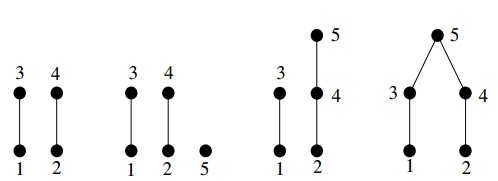
\includegraphics[width=0.8\linewidth]{png/algemtree.png}
        \caption{Updating the forest during the processing of 
        the final column of Figure \ref{fig::emtree}}
        \label{fig::algemtree}
    \end{figure}
\end{exm}

\begin{lem}
    Having constructed the elimination tree, we may use it to 
    factorize the matrix, or another matrix with the same 
    soarsity pattern. We visit the nodes in some topological 
    order (basicly from leaves to root). At each node, we add 
    together the original `elements' (nonzeros in the pivot's 
    row and column) and the generated element matrices from the
    children (if any), perform the elimination operations with 
    the packed matrix, store the calculated rows of $\mU$, and 
    hold the generated element matrix for use later.
\end{lem}

\begin{exm}
    Actually, when no pivoting is needed, frontal method can 
    be easily generalized to matrices only have symmetric 
    pattern. For example, a matrix like
    $$
    \mA=
    \begin{bmatrix}
        2&0&0&2&1\\
        0&1&-1&0&0\\
        0&-1&0&-2&0\\
        4&0&2&14&0\\
        -6&0&0&0&-2
    \end{bmatrix}.
    $$ 

    When eliminating pivot $1$, we consider the first row and 
    column, which is
    $$
    \mA_1^{(145)}=
    \begin{bmatrix}
        2&2&1\\
        4&0&0\\
        -6&0&0
    \end{bmatrix},
    $$ 
    where $(145)$ represent the nonzero indices. The eliminated matrix 
    will be
    $$
    \mathbf{F}_1^{(145)}=
    \begin{bmatrix}
        2&2&1\\
        2&-4&-2\\
        -3&6&3
    \end{bmatrix}.
    $$ 
    The generated element matrix (contribution block) is
    $$
    \mathbf{CB}_1^{(45)}=
    \begin{bmatrix}
        -4&-2\\
        6&3
    \end{bmatrix},
    $$ 
    which is also called the \textit{Schur complement}. $(45)$ 
    means the generated elements will have contribution when 
    eliminating pivots $4$ and $5$.

    Similarly, when eliminating pivot $2$,
    \begin{align*}
        &\mA_2^{(23)}=
    \begin{bmatrix}
        1&-1\\
        -1&0
    \end{bmatrix},\,
    \mathbf{F}_2^{(23)}=
    \begin{bmatrix}
        1&1\\
        -1&-1
    \end{bmatrix},\\
    &\mathbf{CB}_2^{(3)}=\begin{bmatrix}
        -1
    \end{bmatrix}.
    \end{align*}

    When eliminating pivot $3$, notice that there is a 
    generated element matrix $CB_2^{(3)}$, we add together the 
    original elements and the generated element matrix and get
    \begin{align*}
    &\mA_3^{(34)}=
    \begin{bmatrix}
        -1&-2\\
        2&0
    \end{bmatrix},\,
    \mathbf{F}_3^{(34)}=
    \begin{bmatrix}
        -1&-2\\
        -2&-4
    \end{bmatrix},\\
    &\mathbf{CB}_3^{(4)}=
    \begin{bmatrix}
        -4
    \end{bmatrix}.
    \end{align*}
    Similarly, when eliminating pivot $4$, there are generated 
    element matrices $CB_1^{(45)}$ and $CB_3^{(4)}$, so
    $$
    \mA_4^{(45)}=
    \begin{bmatrix}
        6&-2\\
        6&3
    \end{bmatrix},\,
    \mathbf{F}_4^{(45)}=
    \begin{bmatrix}
        6&-2\\
        1&5
    \end{bmatrix},\,
    \mathbf{CB}_4^{(5)}=
    \begin{bmatrix}
        5
    \end{bmatrix}.
    $$ 
    Finally, $\mA_5^{(5)}=3=\mathbf{F}_5^{(5)}$ and the 
    factorization is complete. The elimination tree is as in 
    Figure \ref{fig::exmemtree}.
    \begin{figure}[H]
        \centering
        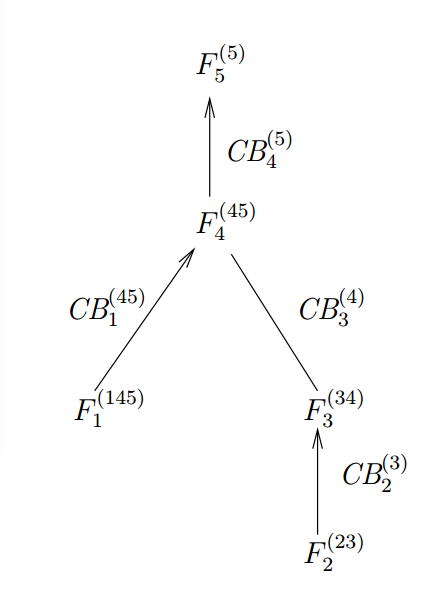
\includegraphics[width=0.5\linewidth]{png/exmemtree.png}
        \caption{Elimination tree}
        \label{fig::exmemtree}
    \end{figure}
\end{exm}

\subsection{Numerical pivoting}
\begin{alg}
    The frontal methods can also be applied to systems which 
    need numerical pivoting. As shown in Figure 
    \ref{fig::pivotfrontal}, where the block of the front 
    that is partially summed is labelled $ps$ and the parts 
    that are fully summed are labelled $fs$. Any entry whose 
    row and column is fully summed (that is, any entry in block 
    $(1,1)$ of Figure \ref{fig::pivotfrontal}) may be used as a 
    pivot. We can use any pivoting strategy including partial 
    pivoting, threshold pivoting and so on. Notice that if 
    unsymmetric interchanges are included, the index list for 
    the rows in the front will differ from columns and will 
    require separate storage.
    \begin{figure}[H]
        \centering
        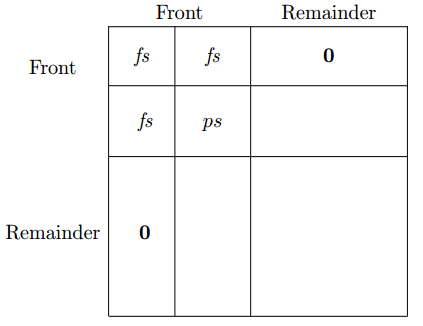
\includegraphics[width=0.8\linewidth]{png/pivotfrontal.png}
        \caption{Reduced submatrix after an assembly and prior 
        to another set of eliminations}
        \label{fig::pivotfrontal}
    \end{figure}

    It is possible that we cannot choose pivots for the whole 
    of the frontal matrix because of small entries in the front 
    or large off-diagonal entries that lie outside the block of 
    the fully-summed rows and columns (that is, because they 
    lie in block $(1,2)$ or block $(2,1)$ of Figure 
    \ref{fig::pivotfrontal}). In this case, we simply leave the
    variables in the front, continue with the next assembly, 
    and then try again. It is always possible to complete the 
    factorization using this pivotal strategy because each 
    entry eventually lies in a fully-summed row and in a 
    fully-summed column.
\end{alg}


\end{multicols} 

\bibliography{ref.bib}
%\bibliographystyle{abbrv}
\bibliographystyle{abbrvnat}
\setcitestyle{authoryear,open={[},close={]}}

\end{document}
%%% Local Variables:
%%% mode: latex
%%% TeX-master: t
%%% End:
